\section{Implementation}
\label{sec:grust:implem}

This section presents the implementation of \GRust, tailored to the automotive software manufacturer
\ampere.
%
It details the design principles, compiler architecture, and technical implementation
choices, highlighting how \GRust achieves predictable and efficient behavior through a combination
of Functional Reactive Programming (with \GRFRP) and Synchronous Programming (with \GRSync).

\subsection{Requirements for Automotive Software}
\label{sec:grust:implem:requirements}

For \GRust to serve as a viable proof of concept for \ampere, it must satisfy several key
requirements rooted in the demands of the automotive industry and the specific challenges of the
\sdv transition. This section outlines the foundational requirements that form the context for our
work. It first recalls the objectives of the thesis, then details the strict safety constraints
imposed by the \iso standard and the new architectural demands of the Software-Defined Vehicle.


\subsubsection{Recalling the Context and Objectives}
\label{sec:grust:implem:recap}

Before detailing the design principles of the \GRust compiler, this section briefly
recapitulates the context and objectives presented in the introduction. We revisit the
challenges of the \sdv transition and restate the goals of \GRust in addressing them.

The automotive industry, including \ampere, is transitioning toward a
\emph{Software-Defined Vehicle} (\sdv) architecture to support advanced computational
features. This shift from distributed \ecus to centralized computers introduces new
challenges for software development. Traditional model-based tools that generate periodic
\Ci code are ill-suited for the dynamic, event-driven workloads of \sdv{}s, leading to
inefficient execution, a heavy burden of manual optimization, and costly verification.

To meet these demands, \ampere is adopting \Rust for its strong safety guarantees and
performance. However, \Rust is a low-level language, creating an abstraction gap for
control engineers accustomed to model-based design. Existing academic paradigms and
industrial tools do not fully bridge this gap. Synchronous languages like \Lustre lack
native support for event-driven behavior and integration with \Rust, while \frp
prioritizes expressivity over the predictability required for critical systems.

\GRust is designed to fill this gap. It provides a high-level, dataflow modeling
language that synthesizes the strengths of established paradigms. The goal of \GRust is
to combine the deterministic, step-based computation of synchronous models with the
expressiveness of \frp for asynchronous, event-driven behavior. By doing so, \GRust
enables engineers to design complex reactive systems at a high level of abstraction
while generating safe, efficient, and asynchronous \Rust code suitable for modern \sdv
platforms.

\subsubsection{Software Requirements of \iso}
\label{sec:grust:implem:design_principles:iso}

A foundational principle for \GRust is its alignment with the \iso safety standard.
Adherence to this standard is not optional in the automotive industry; it is a
prerequisite for developing safety-critical software. Therefore, the design of any new
language or toolchain must be fundamentally guided by the requirements that \iso imposes.
This section outlines the key software-level principles that serve as the benchmark for
any modern development approach. These principles can be grouped into four main pillars:
unambiguous design, safe implementation, rigorous verification, and qualified tools.

\paragraph{Unambiguous Specification and Traceability}
\iso (Part 6) mandates that software be built on a clear, hierarchical architecture with
unambiguous design specifications. For high \Asil levels, it highly recommends using
modeling or semi-formal notations to prevent ambiguity. Furthermore, it requires
bidirectional traceability, allowing auditors to trace a requirement from the
specification down to the code that implements it, and \emph{vice versa}. This is a significant
challenge, as establishing a clear link between an abstract safety goal and a complex
block of low-level, imperative code is often a difficult and manual process.

For instance, a critical aspect of this specification process is defining and verifying real-time
constraints. \iso is a process standard that mandates that such requirements must be \emph{defined,
    justified, and verified}. The actual timing values are derived from system engineering based on
the following.
\begin{description}
    \item[Vehicle dynamics and control theory] The physics of the vehicle
          determine the required reaction times. For example, an ABS controller must
          modulate the brakes at a certain frequency to prevent wheel lockup.
    \item[Fault tolerance time interval (FTTI)] This is the time from the
          detection of a fault until a hazardous event occurs. A timing requirement,
          such as ``send a heartbeat message every 1s'' is derived from the FTTI. If the
          FTTI for a service failure is 500ms, the system must be able to detect the
          absence of the heartbeat and react well within that window.
\end{description}
The \iso process forces these system-level needs to be translated into verifiable
Technical Safety Requirements (TSRs) with concrete timing values. The challenge,
therefore, is not only to specify these timing constraints but to implement and verify
that the software meets them under all operating conditions.

\paragraph{Safe Implementation \via Coding Guidelines}
A cornerstone of software implementation under \iso is adherence to a strict set of
coding guidelines. For languages like \Ci and \Cpp, this requirement is most commonly
fulfilled by adhering to the \emph{Motor Industry Software Reliability Association}
(MISRA) guidelines. As the \defacto industry standard, MISRA defines a safe subset of
\Ci/\Cpp, explicitly forbidding features that are error-prone, ambiguous, or have undefined
behavior. The goal is to produce highly predictable, robust, and maintainable code. The
core principles of such a safe subset are detailed below.

\subparagraph{Deterministic Memory Management}
To ensure predictable temporal behavior and prevent runtime failures, all memory resources
must be managed deterministically. This principle directly forbids the use of dynamic
heap allocation at runtime (\eg \via \texttt{malloc} or \texttt{free}). The rationale is
threefold: first, the time required to allocate memory is non-deterministic, making it
impossible to guarantee worst-case execution times. Second, allocation can fail if the
system runs out of memory (resource exhaustion), a failure mode that is difficult to
handle safely in all parts of a complex application. Third, repeated allocation and
deallocation can lead to memory fragmentation, where the heap has enough free space
overall but not in a single contiguous block, causing future allocations to fail.
Therefore, all memory must be statically allocated at compile time or pre-allocated from
a managed pool before the main operational phase of the software begins.

\subparagraph{Strict Pointer and Spatial Memory Safety}
Preventing memory corruption is one of the highest priorities. This is achieved by
enforcing strict spatial memory safety, meaning that every memory access must be provably
within the bounds of the intended memory object. Consequently, practices that could
violate this are strictly forbidden. This includes most forms of pointer arithmetic, as
it can easily lead to pointers that reference arbitrary memory locations. Most
importantly, it forbids the dereferencing of null pointers and dangling pointers (pointers
that refer to memory that has already been freed). Violations in this category, such as
buffer overflows and use-after-free errors, are the source of the most severe and
notorious safety and security vulnerabilities in software history.

\subparagraph{Elimination of Undefined Behavior}
To guarantee that a program is fully predictable and portable across different compilers
and hardware, its behavior must be completely defined by the language specification. Any
operation that the \Ci/\Cpp standard describes as \emph{undefined} breaks the contract between
the programmer and the compiler, granting the compiler license to generate arbitrary and
unpredictable code. For this reason, all sources of undefined behavior must be
eliminated. This includes using variables before they have been initialized, signed
integer overflow (which can be optimized away by compilers in unexpected ways), and
bit-shifting by an amount greater than or equal to the width of the type.

\subparagraph{Analyzable Control Flow}
To ensure that software is testable, maintainable, and verifiable, its control flow must
be simple and structured. Complex, \emph{spaghetti-like} control flow makes it impossible for
engineers and static analysis tools to reason about the program's execution path. This
leads to strict rules, such as forbidding the use of the \texttt{goto} statement.
Furthermore, unbounded recursion is banned because it introduces the risk of stack
overflow, and it is generally impossible to statically determine the maximum stack depth
of a recursive function.

\subparagraph{Concurrency Safety}
With the prevalence of multi-core processors in modern \ecus, managing concurrency safely
is a critical concern. The primary goal is to prevent data races, which occur when
multiple threads access the same memory location without synchronization and at least one
of those accesses is a write. Data races are another form of undefined behavior and can
lead to silent data corruption. Therefore, coding guidelines for concurrent systems
mandate that all access to shared data must be protected by synchronization mechanisms,
such as mutexes or atomic operations.

These rules, while comprehensive, only address the implementation phase. Enforcing them
in traditional languages requires expensive external tools and rigorous manual discipline.
Furthermore, they are only one part of the overall safety picture, which also includes
unambiguous design (explained above), formal verification, and tool qualification (both explained
below).

\paragraph{Rigorous Verification}
The standard requires extensive verification to ensure software correctness. For high-ASIL
systems, it goes further by highly recommending the use of \emph{formal methods} to
mathematically prove the absence of specific runtime errors, such as division by zero,
numeric overflows, or dead logic. The challenge lies in making such advanced verification
techniques practical and accessible to development teams, as applying them directly to
large, handwritten codebases requires specialized expertise.

\paragraph{Confidence in the Software Toolchain}
Finally, \iso (Part 8) governs the development tools themselves. It requires that all
tools, including compilers and code generators, be \emph{qualified}. This involves a
rigorous process to demonstrate that the tool is fit for its purpose and does not
introduce errors. Tool qualification is a prohibitively expensive effort, creating a
massive barrier to the adoption of new, unqualified tools in a production environment.

Together, these four pillars---an unambiguous design (with verifiable real-time constraints), an
inherently safe implementation, accessible formal verification, and a feasible path to
tool qualification---form the comprehensive set of challenges that guided the design of
\GRust.

\subsubsection{Execution Requirements of the \sdv Architecture}
\label{sec:grust:implem:requirements:sdv}

Beyond safety standards, the shift to the \sdv architecture forces a re-evaluation of the
fundamental execution model used in automotive software. This involves navigating the classic
trade-off between traditional \emph{pull-based} (or demand-driven) and modern \emph{push-based}
(or event-driven) execution strategies, especially in the context of high-bandwidth data processing
and network communication.

The classic automotive approach is pull-based, where components operate on a fixed periodic
schedule. The primary strength of this model is \emph{predictability}. System behavior is easy to
analyze, verify, and test, as all interactions happen at predefined points in time. However, in the
data-rich environment of an \sdv, this model leads to four major inefficiencies:
\begin{description}
    \item[Wasted CPU cycles] Components re-compute their logic at every tick,
          even if no new input data has arrived.
    \item[Communication bus saturation] Data is often transmitted at a fixed
          rate, regardless of whether its value has changed, flooding the network with
          redundant messages.
    \item[Increased latency] The reaction to a critical event is delayed until
          the next sampling instant, introducing a worst-case latency of one full period.
          Meeting strict timing requirements forces the use of very short periods, which
          exacerbates the other two problems.
    \item[Implicit and brittle time-based logic] The periodic model encourages
          engineers to implement time-dependent logic by counting execution ticks rather
          than using explicit timers. For instance, a debouncing filter might be implemented
          by checking if a signal remains stable for 10 consecutive sampling instants.
          This practice creates a fragile and implicit coupling between the functional
          logic and the system's scheduling configuration. If a system integrator later
          changes the component's execution period from 10ms to 20ms for optimization,
          the debouncing logic silently doubles its effective duration from 100ms to 200ms,
          potentially violating system requirements. This makes the software non-portable
          and difficult to maintain, as its correctness depends on an external parameter
          not visible in the component's source code.
\end{description}

To overcome these issues, there is a strong trend toward a push-based strategy. In a push-based
system, computations are initiated only in response to significant events, such as the arrival of
new sensor data. This approach reduces redundant computations, minimizes bus traffic, and
significantly lowers average-case latency.

However, a purely push-based model introduces its own critical safety challenge:
\emph{unpredictability under load}. A faulty sensor or an unusual environmental condition could
trigger an \emph{event storm}---a high-frequency burst of events that overwhelms the system. This
can lead to unbounded CPU usage, memory exhaustion from event queuing, and a failure to process
high-priority events in a timely manner.

Therefore, the ultimate requirement is not to simply choose one paradigm over the other. The core
challenge for a modern automotive language is to \emph{provide a unified framework that safely
    combines the predictability of the pull-based world with the efficiency of the push-based
    world}. A language must enable developers to harness the responsiveness of push-based systems
while providing the necessary control constructs---including explicit handling of time---to manage
event flows, prevent storms, and guarantee predictable behavior under all conditions. This hybrid
push/pull capability is a central requirement for \GRust.

\subsection{The Design Principles of \GRust}
\label{sec:grust:implem:design_principles}

The development of \GRust is guided by a set of core design principles that
address the foundational requirements of safety, efficiency, and usability in modern
automotive software. These principles are the strategic choices shaping the
architecture of the language and its compiler, ensuring that \GRust provides an
effective solution to the challenges posed by the \sdv paradigm. The following
sections detail these five key principles.

\subsubsection{High-Level Abstraction for Control Engineers}
\label{sec:grust:implem:design_principles:abstraction}

Developing critical reactive systems requires a high level of abstraction. As detailed in the
introduction (\Cref{cha:intro}), direct implementation in low-level code is difficult and
error-prone. It demands expertise in areas like memory management and concurrency, which are
distinct from the core domain knowledge of control and vehicle dynamics.

The \iso standard reinforces this need by requiring unambiguous specifications and clear,
bidirectional traceability between requirements and code, as detailed in
\Cref{sec:grust:implem:design_principles:iso}. It encourages the use of modeling tools to prevent
ambiguity and simplify the auditing process, which is challenging to achieve with handwritten
low-level code.

To address this abstraction gap, \GRust is designed as a high-level, \emph{Domain-Specific Language}
(\dsl). Its syntax is declarative and based on dataflow models familiar to control engineers from
tools like \Simulink, \Scade, and
\Lustre~\cite{DBLP:conf/popl/CaspiPHP87,DBLP:conf/tase/ColacoPP17}. This approach is
well-established for modeling requirements and generating traceable low-level code.

Furthermore, to meet the push-based execution needs of the \sdv architecture
(developed in \Cref{sec:grust:implem:requirements:sdv}), \GRust integrates concepts from paradigms
that excel at event-driven modeling. It draws inspiration from
\emph{Functional Reactive Programming}~\cite{DBLP:conf/icfp/ElliottH97} (\frp) and libraries like
\ReactiveX~\cite{reactivex}, incorporating their strengths into a framework that remains familiar to
control engineers. The goal is to provide the expressiveness of event-driven models within a
structure that:
1) improves the clarity with regard to the systems requirements, and
2) feels intuitive to users of synchronous tools, thereby lowering the adoption barrier.

This principle allows engineers to focus on the functional logic of the system---\ie the behavior of
dataflows---rather than the low-level complexities of memory management, concurrency, asynchronous
programming, or the \Rust programming language. The resulting models have clear data dependencies
and are reduced to their core logic, making them more concise and readable. This directly improves
design clarity, simplifies safety reviews, and makes traceability from requirements to the model
more straightforward.

\subsubsection{Safety by Construction \via \Rust Compilation}
\label{sec:grust:implem:design_principles:safety_rust}

Most high-level dataflow languages---including for instance \Simulink~\cite{simulink_codegen},
\Velus~\cite{DBLP:conf/pldi/BourkeBDLPR17}, and \LustreC~\cite{lustrec}---generate \Ci code. \Ci is widely used for its
performance and low-level control, and it remains more readable than assembly. However, it provides
no memory safety guarantees by default. While the compilers for these languages are designed to
produce correct code, ensuring the memory safety of the generated \Ci output requires significant
effort. This can be achieved through tool qualification against standards like
MISRA~\cite{simulink_misra}, by inserting assertions into the code for later verification with tools
like \FramaC~\cite{framac,lustrec}, or by formally proving the entire compilation chain to be
correct~\cite{velus}. This work is tedious, and extending the source language with new features
often demands substantial new proofs. For instance, adding array support to \Velus is a complex
research effort, requiring both efficient data structures and new memory safety proofs.

To meet the \emph{Safe Implementation} requirements of \iso
(\Cref{sec:grust:implem:design_principles:iso}) while avoiding these pitfalls, our second design
principle is to achieve \emph{safety by construction}. Rather than generating \Ci code and relying
on external verifiers, \GRust compiles directly to safe \Rust. This strategic choice allows \GRust
to leverage the full power of the \Rust compiler and its \emph{borrow checker}. As a result, \GRust
programs inherit, by construction, guarantees against entire classes of critical errors, including
memory corruption, buffer overflows, and data races, thus fulfilling the spirit of the MISRA
guidelines automatically.

\paragraph{The Borrow Checker in Practice}
The memory-safety model of \Rust is enforced at compile time through three core concepts:
\emph{ownership}, \emph{borrowing}, and \emph{lifetimes}. These rules are what allow \Rust to
guarantee memory safety without a garbage collector~\cite{DBLP:journals/cacm/JungJKD21}.

In \Rust, every value has a single variable that is its \emph{owner}. When the owner goes out of
scope, the value is automatically deallocated. Ownership can be transferred by \emph{moving} a value
from one variable to another. The compiler statically prevents the use of a variable after its value
has been moved.

\begin{lstlisting}[language=Rust]
fn main() {
    let s1 = String::from("hello");
    let s2 = s1; // Ownership of the string is moved from s1 to s2.

    // The following line would cause a compilation error:
    // error[E0382]: borrow of moved value: `s1`
    // println!("s1 is: {}", s1);
}
\end{lstlisting}

To allow access to data without transferring ownership, \Rust uses \emph{references}, a mechanism
known as \emph{borrowing}. The compiler enforces a critical rule: a piece of data can have either
\emph{multiple immutable} (read-only) references or \emph{exactly one mutable} (read-write)
reference, but never both at the same time.

\begin{lstlisting}[language=Rust]
fn main() {
    let mut s = String::from("hello");
    let r1 = &s; // OK: An immutable borrow.
    let r2 = &s; // OK: Multiple immutable borrows are allowed.

    // The following line would cause a compilation error, because `s`
    // is already borrowed as immutable.
    // error[E0502]: cannot borrow `s` as mutable
    // let r3 = &mut s;

    println!("{} and {}", r1, r2); // r1 and r2 are used here.
}
\end{lstlisting}
This rule, checked at compile time, makes data races impossible by design. Finally, the compiler
uses a system of \emph{lifetimes} to ensure that all references are valid and do not outlive the
data they point to, preventing dangling pointers.

\paragraph{Abstraction with Traits}
Beyond memory safety, \Rust provides powerful, zero-cost abstractions through \emph{traits}. A trait
defines a set of methods that a type must implement to offer certain functionality, similar to an
interface in other languages. This enables polymorphism, allowing developers to write generic code
that operates on any type that implements a given trait. For example, developers could define a
\texttt{Diagnosable} trait for any component that can report its status.

\begin{lstlisting}[language=Rust]
// Define a trait for components that can report a diagnostic status.
pub trait Diagnosable {
    fn report_status(&self) -> String;
}

// Implement the trait for a brake sensor component.
pub struct BrakeSensor {
    pub wheel_location: String,
    pub pressure: u32, // Pressure in PSI
}
impl Diagnosable for BrakeSensor {
    fn report_status(&self) -> String {
        format!("Brake Sensor ({}): Pressure = {} PSI",
                self.wheel_location, self.pressure)
    }
}

// Implement the trait for an engine control unit.
pub struct EngineControlUnit {
    pub has_fault: bool,
    pub fault_code: u16,
}
impl Diagnosable for EngineControlUnit {
    fn report_status(&self) -> String {
        if self.has_fault {
            format!("ECU Fault Detected: Code P{:04X}", self.fault_code)
        } else {
            String::from("ECU Status: OK")
        }
    }
}

// A generic function that runs diagnostics on any compatible component.
pub fn run_system_check<T: Diagnosable>(component: &T) {
    println!("Checking component... Status: {}", component.report_status());
}
\end{lstlisting}
This allows a single function, \texttt{run\_system\_check}, to operate on any component,
from a simple sensor to a complex ECU, as long as it implements the \texttt{Diagnosable}
trait. Traits are a cornerstone of \Rust, enabling modular and reusable code without
sacrificing performance.

\paragraph{The \Rust Toolchain and Ecosystem}
The safety and abstraction capabilities of \Rust are supported by a mature toolchain. Development is
managed by \texttt{cargo}, the official build tool and package manager, which handles dependency
management, compilation, and testing. Reusable libraries, called \emph{crates}, can be shared and
downloaded from a central repository, \texttt{crates.io}. This fosters a rich ecosystem of
high-quality components. Another key feature is the use of \emph{macros} for meta-programming.
Macros are functions that write code during the compilation process; they are identified by a bang
(\texttt{!}), as in \texttt{println!}. They allow for powerful, compile-time code generation that
reduces boilerplate and enhances expressiveness.

\paragraph{Managing Unsafe Code}
Together, these mechanisms provide a strong foundation for memory and concurrency safety. However,
certain low-level operations, such as interfacing with hardware or implementing synchronization
primitives like mutexes, require capabilities that cannot be proven safe by the compiler's rules
alone. For these cases, \Rust provides the \texttt{unsafe} keyword, which allows developers to
bypass some of the compiler's restrictions within a delimited block of code.
%
Using \texttt{unsafe} does not disable all safety checks, but it does place the onus on the
programmer to manually uphold the language's safety invariants. To manage this responsibility
formally, the academic community has developed frameworks for verifying \texttt{unsafe} code. The
\RustBelt project~\cite{DBLP:journals/pacmpl/0002JKD18}, for example, provides a formal foundation
in the \Rocq proof assistant~\cite{rocq} for proving that safe abstractions built on top of
\texttt{unsafe} code are, in fact, sound. This allows for the creation of verified, low-level
libraries---such as a correct(ed) mutex implementation~\cite{rustbelt_mutex_proof,rust_mutex_issue}%
---that can be used from safe \Rust code without compromising the overall safety of the program.

\paragraph{Extensibility with Safe Functions}
A key challenge for any \dsl is extensibility, as developers frequently need to incorporate external
functionalities (such as mathematical libraries or specialized algorithms). In systems that generate
\Ci code, calls to external libraries create a gap in the safety argument, as these components lie
outside the scope of the verification process. \Rust addresses this through its package manager and
rich ecosystem. Since the ecosystem is built around the same principles of safety, developers can
import external \emph{crates} with a high degree of confidence. By compiling to \Rust, \GRust builds
upon this robust foundation, ensuring that complex, performance-critical components can be
implemented and extended with a high degree of confidence.

\subsubsection{Efficient and Safe Execution \via Asynchronous \Rust}
\label{sec:grust:implem:design_principles:async_rust}

As explained in \Cref{sec:intro:gap} of \Cref{cha:intro}, \ampere is adopting asynchronous \Rust to realize the
push-based execution model required by the \sdv architecture. However, direct implementation in a
low-level language like \Rust is challenging, and the complexities of asynchronous programming
further increase the risk of errors. \GRust addresses this by automatically generating safe and
efficient asynchronous \Rust code from a high-level model. This choice is a foundational decision
that directly addresses the challenge of building highly concurrent and resource-efficient software
without sacrificing safety.

Implementing a scalable, push-based system capable of handling thousands of concurrent data sources
presents a significant challenge. Asynchronous \Rust provides the resource efficiency of
non-blocking I/O while maintaining a readable, linear control flow analogous to threaded code. This
is achieved by compiling ergonomic \texttt{async/await} syntax into highly efficient, cooperatively
scheduled state machines, making it the ideal foundation for the \GRust compiler.

The following paragraphs detail the core concepts of this asynchronous model.

\paragraph{The \texttt{async/await} Syntax}
The primary way developers write asynchronous code in \Rust is with the \texttt{async/await}
syntax. This feature allows developers to write non-blocking code that maintains a linear,
readable control flow. An \texttt{async fn} is a function that can be paused and resumed,
and the \texttt{.await} operator is used to non-blockingly wait for a computation to
complete.

Consider a simple asynchronous function that retrieves data from a database:
\begin{lstlisting}[language=Rust]
async fn get_user_permissions(user_id: u64) -> Vec<Permission> {
    // 1. Start execution
    let user = fetch_user(user_id).await;
    // 2. Resume after user is fetched
    let permissions = fetch_permissions(&user).await;
    // 3. Resume after permissions are fetched
    permissions
}
\end{lstlisting}
When this function is called, it does not execute its body and block until completion.
Instead, the compiler transforms the entire function into a self-contained state machine
that implements the fundamental \texttt{Future} trait. Each \texttt{.await} marks a
potential pause point, or a state transition.

The generated state machine for \texttt{get\_user\_permissions} would have roughly three
states:
\begin{description}
    \item[Initial state] The function executes until the first \texttt{.await}.
          It initiates the \texttt{fetch\_user} operation and then, instead of
          blocking, it can yield control, returning a "pending" status. Its local variable
          (\texttt{user\_id}) is saved within the state machine.
    \item[Waiting for permissions] Once the \texttt{user} is fetched, the runtime
          resumes the task. It executes until the next \texttt{.await}, initiating the
          \texttt{fetch\_permissions} operation. It then yields again, now storing both
          the original \texttt{user\_id} and the newly acquired \texttt{user} in its state.
    \item[Final state] Once the \texttt{permissions} are fetched, the task is
          resumed a final time. It runs to completion, returning the final value. The state
          machine is now considered "done".
\end{description}
This transformation allows a single thread to juggle thousands of such tasks, making
progress on each one as its awaited data becomes available.

\paragraph{The \texttt{Future} Trait}
This state machine generation is powered by the \texttt{Future} trait, the core building
block of \Rust's asynchronous ecosystem. A \texttt{Future} represents a value that may not
be ready yet. It has a single method, \texttt{poll}, which an executor calls to drive the
state machine forward. The \texttt{poll} method can return one of two states:
\begin{description}
    \item[\texttt{Poll::Pending}] The value is not yet available. This signals to the
          executor that the task should be suspended and polled again later.
    \item[\texttt{Poll::Ready(T)}] The value of type \texttt{T} is now available, and the
          computation associated with the future is complete.
\end{description}
The \texttt{async/await} syntax is ultimately just convenient syntactic sugar that directs
the compiler to generate a complex, optimized struct with an implementation of this
\texttt{poll} method for us. Each \texttt{.await} call within an \texttt{async} function
corresponds to a point where the generated state machine can pause by returning
\texttt{Poll::Pending} if the awaited value is not yet ready. \texttt{Future}s are also
lazy; they do nothing until they are actively polled by a runtime.

\paragraph{The \texttt{Stream} Trait and Asynchronous Channels}
While a \texttt{Future} represents a single value, the \texttt{Stream} trait represents a
sequence of values arriving over time. It is the asynchronous equivalent of the standard
\texttt{Iterator} trait and is provided by the \texttt{futures} crate.\footnote{A stream's
    \texttt{poll\_next} method can be called repeatedly, yielding a sequence of values wrapped in
    \texttt{Poll::Ready(Some(T))}. It returns \texttt{Poll::Ready(None)} only when the stream is
    exhausted.} The \texttt{StreamExt} trait, implemented for all streams, provides a rich set of
combinator methods (like \texttt{map}, \texttt{filter}) that allow for the declarative composition
of dataflow operations.

This concept maps directly to the dataflow semantics of \GRust. An input to a service
can be modeled as a \texttt{Stream}, and its output can be sent to another task using an
\emph{asynchronous channel}.

For example, a service that converts sensor data and sends alerts could be compiled into an
\texttt{async} function like this\footnote{This function serves as a conceptual illustration of the
    asynchronous pattern. The actual compilation strategy for services is detailed in
    \Cref{sec:grust:implem:choices:frp}.}:
\begin{lstlisting}[language=Rust]
async fn monitor_temperature(
    raw_sensor: impl Stream<Item = f64>,
    mut alert_channel: futures::channel::mpsc::Sender<f64>,
) {
    // Create a new stream that transforms values on the fly.
    let celsius = raw_sensor.map(|raw_val| (raw_val * 100.0) - 50.0);
    // Pin the stream to its location on the stack to iterate over it.
    futures::pin_mut!(celsius);
    // The loop consumes from the transformed stream.
    while let Some(temperature_c) = celsius.next().await {
        if temperature_c > 95.0 {
            // Send a warning to another task via the channel.
            if let Err(_) = alert_channel.send(temperature_c).await {
                // The receiving end has been dropped; stop sending.
                break;
            }
        }
    }
}
\end{lstlisting}
This example showcases several key features of asynchronous dataflow:
\begin{description}
    \item[Stream transformation] The \texttt{.map()} method is a classic example of a stream
          combinator. It takes the original stream and a closure (a function with potentially a
          context), returning a new struct that itself implements the \texttt{Stream} trait. This
          transformation is \emph{lazy}: the conversion logic is not executed immediately. Instead,
          when the new stream is polled (\via \texttt{celsius.next().await}), it internally polls
          the underlying \texttt{raw\_sensor} stream. The closure is applied only when a value is
          received from the source, and the result is yielded. This one-item-at-a-time processing,
          without any intermediate collections or buffers, is what makes the approach highly
          memory-efficient and central to dataflow programming.

    \item[Stream consumption] The loop
          \begin{quote}
              \texttt{while let Some(...) = ... .next().await}
          \end{quote}
          waits without blocking for the next value from the composed \texttt{celsius}
          stream. If the stream is temporarily empty, the entire task is suspended,
          consuming no CPU cycles until a new data point is ready.

    \item[Channels as sinks] The example introduces an asynchronous channel for
          inter-task communication. Channels consist of two halves: a \texttt{Sender} and a
          \texttt{Receiver}. These map directly to the core asynchronous dataflow traits:
          the \texttt{Receiver} implements \texttt{Stream} (a source of data), while the
          \texttt{Sender} implements the \texttt{Sink} trait (a destination for data). The
          call to \texttt{send(...).await} asynchronously sends a value into the channel's
          buffer. The operation is awaited because if the buffer is full, the sending task
          must pause cooperatively until the receiving task consumes a message and makes space.

    \item[Pinning] Finally, the \texttt{futures::pin\_mut!} macro is used because many
          asynchronous types, including the state machines generated by stream combinators,
          cannot be moved in memory once polling has begun. \texttt{Pin} is the type system
          mechanism that enforces this immobility. The macro provides a safe and convenient
          way to pin a value to its stack frame by correctly using \texttt{unsafe} \Rust
          code internally. While this macro is considered sound by the \Rust community, it
          is important to note that its implementation has not been formally proven within a
          framework like \RustBelt.\footnote{After a discussion with X. Denis~\cite{DBLP:conf/pldi/MatsushitaDJD22},
              it was noted that proving this would be a significant challenge, as it would
              require refactoring the underlying formal semantic model to integrate the concept
              of \texttt{Pin}.}
\end{description}
Together, these features provide an elegant and highly efficient toolkit for implementing
complex, reactive, and safe data-driven components.

\paragraph{Asynchronous Runtimes}
In \Rust, objects implementing the \texttt{Future} and \texttt{Stream} traits are best understood as
self-contained blueprints for a computation. For instance, calling an \texttt{async} function does
not immediately execute its code; it returns a \texttt{Future} object. This blueprint bundles the
logic, its current state (\eg which \texttt{.await} point it is paused at), and all its local
variables into a single, inert piece of data.

To execute this plan and drive the state machine forward, an \emph{executor} (or \emph{runtime}) is
required. The fundamental role of a runtime is to manage the lifecycle of asynchronous tasks. It is
responsible for polling them until completion and, most importantly, implementing a \emph{scheduler}
to decide which task to run on which available worker thread. When a future returns \texttt{Pending},
the runtime suspends it and polls other tasks. The key to this entire system is how a suspended task
signals that it is ready to make progress again.

This signaling is achieved through the \texttt{Waker} API. The \texttt{poll} method of a future is
called with a \texttt{Context} argument containing a \texttt{Waker}. A \texttt{Waker} is a handle
that notifies the executor that its associated task should be scheduled to be polled again. The
contract is as follows: if a future returns \texttt{Pending}, it must ensure the \texttt{Waker} is
stored somewhere so that it will be invoked when the task is ready to make progress. This mechanism
works for both external and internal events:
\begin{description}
    \item[External events (I/O)] A task awaiting a network packet registers its \texttt{Waker} with
          the I/O event system of the OS (\eg \texttt{epoll}). When the OS notifies the runtime of
          an event on that socket, the runtime invokes the associated \texttt{Waker}, placing the
          task back in the ready queue.

    \item[Internal events (inter-task)] A task awaiting a channel's \texttt{receive} operation
          stores its \texttt{Waker} with the channel. When another task sends a value to that
          channel, it finds and invokes the stored \texttt{Waker}, signaling the executor to wake
          the receiving task.
\end{description}
This unified \texttt{Waker} mechanism is what allows the entire asynchronous ecosystem to compose
efficiently.

While the \texttt{Future} and \texttt{Waker} APIs are standardized, the \Rust standard library
does not include a runtime. The \Rust community created a rich ecosystem of runtimes, with different
scheduling philosophies, optimized for different workloads.
\begin{itemize}
    \item \texttt{tokio}~\cite{tokio} is the most widely adopted, \defacto standard. It uses a
          multi-threaded \emph{work-stealing scheduler}, where each thread has a local task queue. A
          thread that runs out of work will \emph{steal} tasks from other threads. This provides
          excellent load balancing and high throughput, as threads primarily work on their local
          queues, minimizing contention and improving data locality.

    \item \texttt{async-std}~\cite{async_std} is another popular multi-threaded runtime. Its design
          philosophy prioritizes providing an stable API (mirroring the standard library), without
          depending on non-standard crates like \texttt{futures}.

    \item Others, like \texttt{smol}~\cite{smol}, offer a minimalist and modular design \via a
          collection of smaller, interoperable crates. This allows developers to reduce binary size
          by including only necessary components. Additionally, highly specialized runtimes like
          \texttt{embassy}~\cite{embassy} exist for constrained \texttt{no\_std} embedded systems.
\end{itemize}

For the context of \sdv architectures running on high-performance computing platforms,
\texttt{tokio} seems to be a suitable choice due to its proven performance, maturity, and extensive
library support. It is crucial to acknowledge, however, that its complex scheduler has not been
formally proven correct and uses \texttt{unsafe} code. Verifying such a complex concurrent algorithm
is a challenge. Instead, the \texttt{tokio} team relies on other techniques, like the model checker
\texttt{loom}~\cite{loom}, that can exhaustively explore all possible thread interleavings for a
\emph{given test case}, providing a very high degree of confidence that the implementation is free
of data races and other concurrency bugs.

\paragraph{Conclusion on asynchronous \Rust}
By compiling to asynchronous \Rust, \GRust provides an implementation that is not only memory-safe
and concurrency-safe by construction, but also highly efficient and seamlessly integrated with the
modern runtimes used in performance-critical automotive software.

\subsubsection{Accessible Formal Verification}
\label{sec:grust:implem:design_principles:verif}

The \iso standard highly recommends formal methods for verifying high-\Asil systems. However, the
practicality of this recommendation depends heavily on the chosen implementation language and its
verification ecosystem.

Verifiers for \Ci, such as \FramaC, operate on low-level code. Before proving a high-level
functional property (\eg that a filter output is always within a certain range), programmers must
discharge a heavy proof burden related to memory safety. This involves manually annotating code with
assertions to prove that pointers are valid, do not alias (point to overlapping memory), and that
all memory accesses are within bounds. This process is tedious, error-prone, and requires deep
expertise in formal methods.

In contrast, verifiers for \Rust, such as \Creusot, benefit from a significant advantage. The \Rust
compiler borrow checker already proves the absence of entire classes of errors, including data races
and memory violations. By enforcing these properties at compile time, \Rust allows the verifier and
the programmer to focus exclusively on the \emph{functional correctness} of the program logic. The
complex proofs about pointer validity that dominate \Ci verification are simply not necessary.

\GReusot leverages this advantage while preserving the high-level abstraction of \GRust. Since
\Creusot operates on plain \Rust code, a gap exists between the abstract \GRust model and the
generated code. \GReusot bridges this gap by allowing developers to write safety properties directly
within their \GRust models. The compiler then automatically translates these high-level
specifications into the corresponding \Creusot annotations on the generated \Rust code. This
approach makes formal verification an integral part of the development workflow, enabling engineers
to prove critical properties at a level of abstraction that matches the design.

\subsubsection{Tool Qualification}
\label{sec:grust:implem:design_principles:qualif}

The \iso standard (Part 8) requires that development tools, including compilers, undergo a rigorous
\emph{tool qualification} process. This process is notoriously expensive and time-consuming,
creating a significant barrier to the adoption of new tools in safety-critical environments. Our
implementation strategy is designed to provide a pragmatic and cost-effective path to qualification.

The \GRust compiler prototype is not a standalone compiler that generates machine code. Instead,
it is implemented as a \Rust \emph{procedural macro}. A procedural macro is a special type of
function executed by the compiler before the borrow checker, which takes a stream of code tokens as
input and produces a new stream of tokens as output. In our case, the macro transforms the
high-level \GRust syntax into standard, safe \Rust code during compilation. This code follows the
rest of the compilation scheme of \Rust, including the borrow checker.

This source-to-source translation architecture dramatically simplifies the qualification argument.
The responsibility for generating correct machine code is delegated to the \Rust compiler itself.
The qualification effort for \GRust can therefore focus on a much smaller scope: proving that the
procedural macro correctly translates any valid \GRust program into a \emph{safe} \Rust program.

This strategy becomes particularly powerful when combined with an officially qualified \Rust
toolchain. \ferrocene is the first \Rust compiler toolchain qualified for use in \iso \Asil~D and
other safety-critical domains. By generating standard \Rust code, \GRust is designed to be fully
compatible with \ferrocene. This allows the \GRust compiler to rely on the existing qualification of
\ferrocene, limiting the new qualification effort to the \GRust-to-\Rust translation step. This
approach makes tool qualification a feasible goal, positioning \GRust as a viable candidate for
industrial adoption.

\subsubsection{Summary}
\label{sec:grust:implem:design_principles:summary}

In summary, the design of \GRust is founded on five interconnected principles that collectively
address the challenges of developing software for \sdv architectures. First, a \emph{high-level,
    domain-specific abstraction} makes the language intuitive for control engineers. Second,
\emph{safety by construction} is achieved by compiling to safe \Rust, which eliminates entire
classes of memory and concurrency errors. Third, compilation to \emph{asynchronous \Rust} ensures
efficient, scalable, and push-based execution suitable for dynamic workloads. Fourth,
\emph{accessible formal verification} is integrated into the workflow, allowing engineers to prove
functional correctness at the model level. Finally, a pragmatic approach to \emph{qualification}
simplifies the path to certification by leveraging the existing \Rust ecosystem.\footnote{Tool
    qualification is out of the scope of this thesis. But it is an important point to address in
    this domain.} Together, these principles create a robust framework for building reliable and
maintainable automotive systems.

\subsection{Implementation Choices}
\label{sec:grust:implem:choices}

Building upon the design principles established in \Cref{sec:grust:implem:design_principles}, this
section develops the implementation of the \GRust prototype compiler. We first examine its
high-level architecture, focusing on the decision to build it as a \Rust procedural macro and the
implications of this choice. We then focus on the specific compilation pipelines for the two
sub-languages, \GRSync and \GRFRP, detailing the sequence of analyses and transformation passes that
convert high-level, declarative models into safe and efficient asynchronous \Rust code.

\subsubsection{Prototype Compiler Architecture}
\label{sec:grust:implem:choices:architecture}

This section details the architecture of the prototype compiler for \GRust. The implementation
follows the design principles outlined previously. The complete source code for the compiler is
publicly available in the \GRust repository:
\begin{center}
    \URLgrust
\end{center}
A (work in progress) documentation, including user guides and language references, is provided in
the \GRust Book:
\begin{center}
    \URLgrbook
\end{center}

\paragraph{Compiler as a Procedural Macro}

As introduced in \Cref{sec:grust:implem:design_principles:qualif}, the \GRust compiler prototype is
implemented as a \Rust \emph{procedural macro}. This architectural choice favors usability and
integration with the \Rust ecosystem over the traditional approach of a \emph{standalone
    executable}.

A standalone compiler, such as \texttt{gcc}, is a separate command-line program. This model would
require a multi-step workflow: developers would write a \GRust model in a dedicated file (\eg
\texttt{model.gr}), run an external compiler to generate an intermediate \Rust file (\eg
\texttt{model.rs}), and then manually integrate that artifact into a larger \Rust project. Such a
process complicates the compilation system and burdens the developer with managing the resulting
artifacts, a task that often necessitates custom tooling.

In contrast, a procedural macro integrates the \GRust compiler directly into the standard \Rust
compilation process. A procedural macro is a function that transforms code during compilation. It
executes after the source text has been parsed into a stream of tokens but before static analysis
phases like type checking or borrow checking. The macro takes the token stream inside its
invocation, processes it, and produces a new stream of tokens representing standard \Rust code. The
output stream is inserted back into the full program token stream, for processing by the subsequent
stages of the \Rust compiler.

In essence, the \GRust compiler acts as a source-to-source translator, that is seamlessly invoked by
the \Rust compiler. It converts the high-level \GRust syntax into standard, safe \Rust code that is
then validated by the borrow checker.

This approach offers several key advantages that align with the design goals of \GRust.
\begin{description}
    \item[Seamless Integration] The compiler integrates directly into the standard \Rust toolchain.
          Developers use familiar commands like \texttt{cargo build} and \texttt{cargo check},
          without external build scripts or pre-processing steps, resulting in a smooth and
          idiomatic developer experience.

    \item[IDE and Tooling Support] Since \GRust code resides within \Rust files, it immediately
          benefits from the existing \Rust ecosystem. Developers gain syntax highlighting and
          auto-completion from tools like the \Rust Language Server. Furthermore, compilation errors
          from later stages, including type and borrow checking, are mapped directly back to the
          original \GRust source code. (Though there is limited control on the shape of these
          errors, see the cons of the approach.)

    \item[Interoperability and Code Reuse] \GRust models can directly use standard \Rust
          definitions, such as types and functions, enabling straightforward integration with
          existing codebases. This design also fosters a modular ecosystem of reusable libraries.
          The \GRust standard library, \texttt{grust-std}, exemplifies this by offering common
          components for mathematical operations (\eg \texttt{sin}, \texttt{cos}) and numerical
          algorithms, often by wrapping functions from the \Rust standard library. For convenience,
          it is re-exported by the main \texttt{grust} crate, making its components accessible
          through the path \texttt{grust::std}.

    \item[Simplified Qualification Path] The qualification effort can focus on verifying the
          correctness of the source-to-source transformation performed by the macro, rather
          than an entire compiler toolchain. When combined with a qualified \Rust compiler
          like \ferrocene, this approach offers a pragmatic path toward meeting \iso
          requirements.
\end{description}

Despite its benefits, the procedural macro approach also presents certain challenges.
\begin{description}
    \item[Diagnostic Quality] This diagnostic challenge is best illustrated with a concrete example.
          Consider a type mismatch between two services:
          \begin{itemize}
              \item A \texttt{speed\_sensor} service exports a signal:
                    \begin{lstlisting}[language=GRust,numbers=none,basicstyle=\ttfamily\color{BlackText}]
export signal speed: float;
\end{lstlisting}
              \item A \texttt{cruise\_control} service imports this signal with the wrong type:
                    \begin{lstlisting}[language=GRust,numbers=none,basicstyle=\ttfamily\color{BlackText}]
import signal speed: int;
\end{lstlisting}
          \end{itemize}
          A standalone compiler would parse the entire project, recognize the mismatch, and report
          a clear, high-level error, such as:
          \begin{quote}
              Type mismatch for signal \texttt{speed}: exported as \texttt{float} but imported as
              \texttt{int}.
          \end{quote}
          In contrast, the procedural macro lacks this global view. To illustrate the consequence,
          let us assume a compilation model where each flow corresponds to a \Rust channel.%
          \footnote{While the actual compilation strategy differs, it does not resolve this issue.}
          The macro would process each service in isolation, generating code for a channel of type
          \texttt{f64} in one case and \texttt{i64} in the other. The error is only caught later by
          the \Rust compiler itself, which would report a lower-level message like:
          \begin{quote}
              mismatched types: expected \texttt{Receiver<i64>}, found \texttt{Receiver<f64>}.
          \end{quote}
          The developer must then work backward from this \Rust-specific error to diagnose the
          logical mistake in the \GRust model. This issue is inherent to the source-to-source
          translation approach.

    \item[Isolated Compilation and Interface Safety] Each procedural macro invocation runs in
          isolation, which prevents components from being shared directly between compilation
          units and thus complicates modular design. To bridge this gap, the compiler generates
          code that conforms to a public \texttt{Component} trait, creating a stable interface.
          This approach, however, creates a safety loophole: developers can manually implement this
          trait, bypassing the checks of the compiler and violating the semantic guarantees that
          \GRust is designed to provide.

          % \item[Lack of Semantic Context] Procedural macros operate on a purely syntactic token
          %       stream, before the \Rust compiler performs its semantic analyses phases, such as type
          %       checking. As a result, the macro lacks access to the compiler's rich type
          %       information. To enforce its own correctness rules, the \GRust compiler must
          %       therefore perform its own name and type resolution, effectively re-implementing a
          %       portion of the \Rust compiler's work. This approach not only increases the
          %       implementation complexity but also introduces the risk of discrepancies between the
          %       macro's analysis and that of the actual \Rust compiler.

    \item[Debugging and Performance Introspection]
          Developers often need to understand the runtime behavior of a program, either to debug its
          logic or to analyze its performance. The macro-based architecture can complicate this,
          as the executable logic resides in the generated \Rust code, not the original model.
          To provide visibility without requiring manual inspection of the generated code, \GRust
          integrates two key features from the \Rust ecosystem.
          %
          First, for debugging dataflow, a built-in \texttt{log} statement allows developers to
          print the value of any variable within a \GRust component at each execution step.
          This provides a simple, direct way to trace a component's internal state from the
          runtime output.
          %
          Second, for performance analysis, the compiler can instruments the generated \Rust
          functions corresponding to \GRust components and functions. It uses the popular
          \texttt{tracing} crate~\cite{tracing_rust} which captures the runtime duration and
          interactions of each high-level component.
          %
          Together, these features provide essential introspection, enabling developers to debug
          and profile their models effectively at the source level.

    \item[Impact on Compilation Time] The execution of the procedural macro adds to the overall
          compilation time, as it involves parsing the \GRust syntax, performing semantic analyses,
          and generating code. While this overhead can be a concern for large projects, empirical
          evaluation suggests that the \GRust macro does not constitute a significant bottleneck.
          The time spent within the macro is marginal compared to the more computationally intensive
          phases of the \Rust compiler that follow. Therefore, the impact on build times is
          considered a reasonable trade-off for the high-level abstractions and safety guarantees
          that the language provides.
          %
          It is worth noting that achieving this performance profile was an iterative process. For
          instance, the initial generation of \Rust tokens involving the \texttt{syn}
          crate~\cite{syn_rust} led to exponential compile times. A subsequent issue was identified
          in the algorithm for resolving service imports, which had a complexity exponential in the
          number of imported flows. This made compilation prohibitively slow for services with more
          than ten imports. Both of these performance regressions were identified and resolved.
\end{description}

\newpage

\paragraph{Macro Usage and Configuration}

The \GRust compiler is invoked through the \texttt{grust!} procedural macro, which is available in
the main \texttt{grust} crate. Developers write \GRust logic directly inside a \Rust file within
the macro call, as illustrated in the following example.

\begin{lstlisting}[
    language=GRust,
    label=lst:grust:implem:choices:architecture:usage:example,
    caption={[Usage of the \texttt{grust!} macro.]%
    Defining a hazard light controller service with the \texttt{grust!} macro.},
    captionpos=b
]
grust::grust! {
    #![mode = test, tracing, dump = "path/to/file.rs"]
    // Import an event that occurs when the physical hazard light button is pressed.
    import event hazard_button_pressed: unit;

    // Export a boolean signal representing the desired state of the hazard lights.
    export signal hazard_lights_on: bool;

    // A stateful component that implements a toggle (a T-flip-flop).
    // It flips its boolean state every time it receives a 'trigger' event.
    component toggle(trigger: unit?) -> (state: bool) {
        when {
            init => {state = false;}             // The initial state is `off'.
            trigger? => {state = !(last state);} // When triggered, flip the last state.
        }
    }

    // The service defines the high-level dataflow logic.
    service hazard_light_controller {
        // 1. Define an auto-off event using the `timeout` operator. 
        //    This event fires if `hazard_button_pressed` is not received for
        //    5 minutes (300,000 ms), providing a trigger to turn the lights off.
        let event auto_off_trigger: unit = timeout(hazard_button_pressed, 300000);

        // 2. Combine the manual button press and the auto-off trigger into a
        //    single event stream using the `merge` operator.
        let event combined_trigger: unit = merge(hazard_button_pressed, auto_off_trigger);

        // 3. The output signal is computed by the `toggle` component, which is now
        //    driven by the combined trigger.
        hazard_lights_on = toggle(combined_trigger);
    }
}
\end{lstlisting}

The example in \Cref{lst:grust:implem:choices:architecture:usage:example} defines a service that
models a common automotive pattern: toggling a state (the hazard lights) in response to a discrete
event (a button press) with an automatic shut-off feature to prevent battery drain. The compiler
macro processes this definition and generates the corresponding asynchronous \Rust code.

As shown in the listing, the behavior of the compiler can be configured using
\emph{inner attributes}, which are placed inside the \texttt{grust!} block using the idiomatic \Rust
notation \texttt{\#![...]}. Multiple options can be combined within a single attribute, separated by
commas. The available configuration options are summarized in \Cref{tab:grust:implem:choices:architecture:usage:configs}.

\newpage

\begin{longtable}{
    l % Attribute column
    >{\raggedright}p{0.5\textwidth} % Description column
    l % Default column
    }
    \toprule
    \textbf{Attribute}            & \textbf{Description}                                                             & \textbf{Default}        \\
    \midrule
    \endfirsthead
    % --- Header for subsequent pages ---
    \toprule
    \textbf{Attribute}            & \textbf{Description}                                                             & \textbf{Default}        \\
    \midrule
    \endhead
    % --- Table Content ---
    \multicolumn{3}{l}{\textbf{Compilation Modes}}                                                                                             \\
    \midrule
    \texttt{mode = demo}          & Sets the target to a real-time execution.                                        & \textit{Enabled}        \\
    \texttt{mode = test}          & Test environment with immediate I/O.                                             & Disabled                \\
    \texttt{mode = greusot}       & Generates \Creusot specifications.                                               & Disabled                \\
    \midrule
    \multicolumn{3}{l}{\textbf{Introspection and Debugging}}                                                                                   \\
    \midrule
    \texttt{tracing}              & Instruments generated code with \texttt{tracing} spans for performance analysis. & Disabled                \\
    \texttt{dump = "path"}        & Dumps the generated code to the file path.                                       & Disabled                \\
    \texttt{levenshtein = true}   & Levenshtein suggestions for typos.                                               & Disabled                \\
    \texttt{stats\_depth = N}     & Compilation pass timings up to depth \texttt{N}.                                 & \texttt{0} (Disabled)   \\
    \midrule
    \multicolumn{3}{l}{\textbf{Runtime and Code Generation}}                                                                                   \\
    \midrule
    \texttt{public = B}           & Visibility to public (\texttt{true}) or private (\texttt{false}).                & \texttt{true}           \\
    \texttt{spawn\_with = "..."}  & Specifies the async spawning function.                                           & \texttt{"tokio::spawn"} \\
    \texttt{get\_handle = "..."}  & Type returned by the \verb|run| function.                                        & \verb|()|               \\
    \midrule
    \multicolumn{3}{l}{\textbf{Experimental Parallelization}}                                                                                  \\
    \midrule
    \texttt{para}                 & Enables parallel execution of independent dataflows within services.             & Disabled                \\
    \texttt{align}                & Enforces memory alignment for component states to optimize access.               & Disabled                \\
    \texttt{component\_para(...)} & Configures heuristics for parallelizing computations inside components.          & Disabled                \\
    \texttt{dump\_graph = "path"} & Dumps the component dependency graph to the specified file path.                 & Disabled                \\
    \bottomrule
    \caption[Configuration attributes for the \texttt{grust!} macro.]%
    {Configuration attributes for the \texttt{grust!} macro.}
    \label{tab:grust:implem:choices:architecture:usage:configs}                                                                                \\
\end{longtable}

\paragraph{Overview of the Compiler Architecture}
Before detailing the specific architecture of the \GRust compiler, it is useful to outline the
structure of a typical compiler. A compiler is fundamentally a translator that converts a program
from a high-level source language into a lower-level target language (\eg machine code). This
translation is not a single, monolithic step but rather a multi-stage pipeline, where each stage,
commonly called \emph{pass}, progressively transforms the program representation. This process is
generally divided into two major parts: the \emph{frontend} and the \emph{backend}.

The frontend is responsible for analyzing the source code and verifying its correctness
according to the language rules. This involves several passes:
\begin{description}
    \item[Lexical Analysis (Lexing)] The process begins with the \emph{lexer}, which reads the
          raw source text and groups characters into a sequence of meaningful symbols called
          \emph{tokens}. For instance, the statement \texttt{let x = 10;} would be broken down
          into tokens for the keyword \texttt{let}, the identifier \texttt{x}, the operator
          \texttt{=}, the literal \texttt{10}, and the separator \texttt{;}.

    \item[Syntactic Analysis (Parsing)] The token sequence is fed to the \emph{parser}, which
          verifies its grammatical structure. The output is an \emph{Abstract Syntax Tree} (AST),
          a hierarchical representation of the code. For example, the AST for the statement
          \texttt{let x = 10;} would capture its structure as follows:\footnote{This example retains
              nodes for purely syntactic elements like the \texttt{let} keyword. This is a practical
              choice, as it allows the compiler to store precise location information for each
              token, which is essential for generating meaningful error messages.}
          \begin{center}
              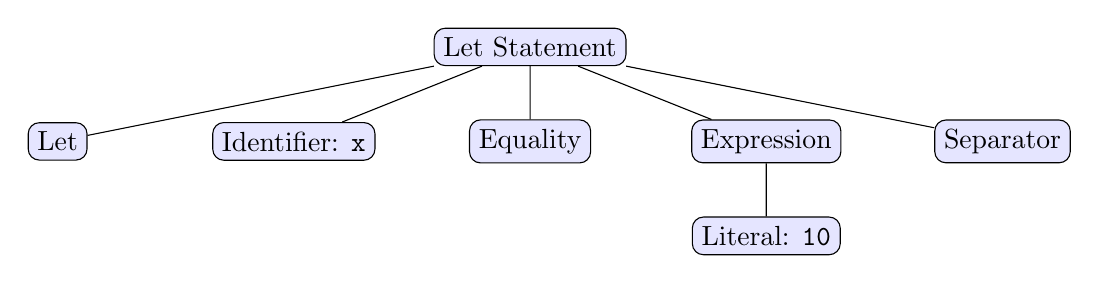
\begin{tikzpicture}[
                      level distance=1.2cm, sibling distance=3cm,
                      treenode/.style = {rectangle, rounded corners, draw, fill=blue!10, align=center}
                  ]
                  \node[treenode] {Let Statement}
                  child { node[treenode] {Let} }
                  child { node[treenode] {Identifier: \texttt{x}} }
                  child { node[treenode] {Equality} }
                  child { node[treenode] {Expression} child { node[treenode] {Literal: \texttt{10}} } }
                  child { node[treenode] {Separator} };
              \end{tikzpicture}
          \end{center}
          The AST captures the program structure but not yet its full meaning.

    \item[Semantic Analyses] This phase traverses the AST to check for semantic correctness,
          enforcing rules that syntax alone cannot capture. This includes \emph{type checking}
          (ensuring that operations are performed on compatible types), verifying that
          variables are declared before use, and resolving the scope of identifiers. During
          this pass, the compiler builds a \emph{symbol table} to store information about
          program identifiers, such as their type and location. The output is often a
          semantically validated and annotated AST.
\end{description}

The backend takes the validated representation from the frontend and generates the final target
code. This process is typically mediated by one or more \emph{Intermediate Representations} (IRs).
An IR is a representation of the program that is lower-level than the source AST but more abstract
than machine code.
%
The use of an IR is a powerful design principle that decouples the frontend from the backend,
reducing the implementation effort from a combinatorial \(M \times N\) to a more manageable
\(M + N\) components. This modularity allows an infrastructure like
\emph{LLVM}~\cite{DBLP:conf/cgo/LattnerA04} to support multiple source languages and hardware
architectures with a shared set of optimizations. In the context of a \dsl, this same
principle enables targeting multiple high-level languages like \Ci, \textsc{Ada}, or \Rust
from a single, common IR.
%
This backend process generally involves two main stages:
\begin{description}
    \item[Optimization] A compiler usually performs transformation passes on the IR to improve
          code performance. The \GRust compiler keeps this stage minimal, as it delegates the
          responsibility of optimization to the highly-advanced \Rust compiler, which operates
          on the generated code. This significantly reduces the implementation complexity of \GRust
          itself.

    \item[Code Generation] Finally, the IR is translated into the target language. In the
          context of \GRust, this stage consists of generating safe and idiomatic \Rust
          source code from the final IR.
\end{description}

The \GRust compiler is designed as a source-to-source translator that follows this approach. It
transforms \GRust source code through a series of dedicated IRs, ultimately generating safe \Rust
code. The subsequent sections detail the design of each of these internal passes.

\paragraph{Structure of the \GRust Compiler}

The \GRust compiler repository is organized as a \Rust \emph{workspace}, a structure that manages a
set of related crates. This modular design separates user-facing elements from the internal compiler
passes, promoting maintainability and clarity. The key crates are detailed below, grouped by their
role in the ecosystem, and illustrated in \Cref{fig:grust:implem:choices:architecture:compilo}.

\begin{figure}[ht!]
    \centering
    
\includegraphics[width=1\textwidth]{compiler_graph.pdf}
    \caption[Architecture of the \GRust compiler.]%
    {The architecture of the \GRust compiler, illustrating the key passes of the compilation
        pipeline from source code to executable.}
    \label{fig:grust:implem:choices:architecture:compilo}
\end{figure}

\subparagraph{User-Facing Crates}
These are the crates developers directly interact with.
\begin{itemize}
    \item \texttt{grust}: The primary, user-facing crate that serves as a facade, consolidating all
          necessary elements for development. It provides the \texttt{grust!} macro, re-exports the
          core and standard libraries (\texttt{grust\_core} and \texttt{grust\_std}), and
          bundles key external libraries such as \texttt{futures}, \texttt{tokio}, \texttt{tracing},
          and \texttt{rayon}. This is the only crate developers need to import.

    \item \texttt{grust-std}: This crate acts as the standard library for \GRust, offering a
          collection of pre-built elements. It includes common mathematical functions and numerical
          algorithms like integrators, which are designed to be compatible with the push-based
          execution model.\footnote{The correctness of time and memory-dependent components, such as
              integrators, is not guaranteed in a push-based system. Consequently, \GRust imposes a
              typing discipline to restrict their usage, a mechanism further explained and formalized in
              \Cref{sec:semantics:grsync:react_typing} of \Cref{cha:semantics}.}
\end{itemize}

\subparagraph{Runtime Support}
This crate provides essential definitions for the generated code.
\begin{itemize}
    \item \texttt{grust-core}: This crate defines the fundamental traits and types required by the
          generated code. This includes the \texttt{Component} trait, which all compiled components
          must implement (\Cref{sec:grust:implem:choices:sync}), and specialized stream types used
          for scheduling inputs and timers in services (\Cref{sec:grust:implem:choices:frp}).
\end{itemize}

\subparagraph{Compiler Infrastructure}
These crates form the foundation of the compilation.
\begin{itemize}
    \item \texttt{grust-proc}: This crate defines the \texttt{grust!} procedural macro. As required
          by \Rust, its manifest (\texttt{Cargo.toml})\footnote{The \texttt{Cargo.toml} file of a
              package is its \emph{manifest}, containing metadata used to compile the package.} is
          configured with \texttt{proc-macro = true}. Its library file, shown below, contains the
          entry point that passes the token stream to the main compiler logic.
          \begin{lstlisting}[language=Rust,numbers=none]
use compiler_top::{handle_tokens, TokenStream};
// The GRust compiler, implemented as a procedural macro.
#[proc_macro]
pub fn grust(tokens: TokenStream) -> TokenStream {
    handle_tokens(tokens)
}
\end{lstlisting}

    \item \texttt{compiler-top}: This crate orchestrates the compilation pipeline. It contains the
          function \texttt{handle\_tokens} that invokes the sequence of analyses and transformation
          passes on the input tokens and returns the generated \Rust code.

    \item \texttt{compiler-common}: A utility crate that defines shared data structures used across
          the entire compiler, including types for representing \GRust operations, error-reporting
          structures, keywords, and graph data structures.
\end{itemize}

\subparagraph{Compiler Passes and Intermediate Representations}
The translation is performed across three internal crates, each corresponding to a pass of
transformation and a specific IR.
\begin{itemize}
    \item \texttt{compiler-ir0}: This pass is responsible for parsing, transforming the raw token
          stream into an AST. The process is built upon the \texttt{syn} crate~\cite{syn_rust}, a
          parsing library. The parser is implemented by defining AST data structures that implement
          the \texttt{Parse} trait. This approach simplifies the development of a parser
          by turning the complex task of implementing a parsing algorithm (like
          LALR~\cite{DBLP:journals/toplas/DeRemerP82}) into the more manageable one of defining the shape of the
          expected code.

    \item \texttt{compiler-ir1}: This pass performs semantic analyses on the AST. This includes type
          checking (it is an implementation of the typing rules from \Cref{sec:grust:typing}),
          dependency graphs generation, causality analysis for components (this is a specific
          analysis that is detailed in \Cref{sec:grust:implem:choices:sync}), and other correctness
          checks and normalization processes. This pass enriches the AST with semantic information,
          preparing it for code generation.

    \item \texttt{compiler-ir2}: The final pass is responsible for code generation. It encodes
          the annotated AST into a target-agnostic IR. This IR models the high-level semantics of
          the program, representing components as state machines and services as import
          propagators.\footnote{This representation is abstract; at this stage, it could
              theoretically be used to generate \Ci or other languages.} The translation of this IR
          into \Rust code is then orchestrated by the \texttt{quote} crate~\cite{quote_rust}. Each
          element in the IR implements the \texttt{ToTokens} trait, which defines how it should be
          rendered as a stream of \Rust tokens. The \texttt{quote!} macro provides a template-like
          syntax that closely resembles the structure of the final \Rust code, making the
          code-generation logic highly readable and maintainable. For instance, the translation of a
          unary operation is defined as follows.
          \begin{lstlisting}[language=Rust]
// IR definition (`Box` is used for recursive types)
struct UnaryOperation { op: UnaryOp, expr: Box<Expression> }
// The implementation that generates Rust code
impl ToTokens for UnaryOperation {
    fn to_tokens(&self, tokens: &mut TokenStream) {
        let UnaryOperation { op, expr } = self;
        quote! { #op #expr }.to_tokens(tokens)
    }
}
\end{lstlisting}
          The code within the \texttt{quote!} macro directly mirrors the target \Rust syntax. The
          \texttt{\#op} and \texttt{\#expr} placeholders are interpolated, which recursively invokes
          the \texttt{ToTokens} implementation for the inner fields. This compositional approach
          allows the entire IR to be translated into a final token stream, which is then returned by
          the procedural macro.
\end{itemize}

The two following sections detail the compilation of the two sub-languages of \GRust, namely \GRSync
and \GRFRP.

\subsubsection{Compilation of \GRSync Functions and Components}
\label{sec:grust:implem:choices:sync}

This section describes the compilation for the two main constructs of the \GRSync
sub-language: functions and components.

\paragraph{Compilation targets}
While both are translated into \Rust code, their compilation targets and the challenges they present
are different.

The compilation of \GRSync functions is straightforward. As these functions are purely combinatorial
and stateless, they map directly to standard \Rust functions. The compiler's role is primarily to
perform semantic checks---such as verifying the correct usage of identifiers (ensuring that they do
not call components) and ensuring type consistency---before generating the equivalent, syntactically
correct \Rust function. Because those analyses are also performed on components, the detailed
explanation of the compilation will be focused on components.

The compilation of a \GRSync component produces three \Rust structs: one for inputs, one for
outputs, and one for the internal state. The state struct implements the \texttt{Component} trait,
which is defined in the \texttt{grust-core} library as follows.
\begin{lstlisting}[language=Rust]
pub trait Component {
    type Input;
    type Output;
    fn init() -> Self;
    fn step(&mut self, input: Self::Input) -> Self::Output;
}
\end{lstlisting}
The \texttt{Self} type refers to the type implementing the trait (the implementor), \texttt{self}
refers to an instance of \texttt{Self}, and \texttt{\&mut self} is a syntactic sugar for
\texttt{self: \&mut Self}.
%
The \texttt{Component} trait defines the framework for a synchronous, stateful computation.
The \texttt{init} function creates an instance of the component in its initial state. The
\texttt{step} function executes a single computational step: from a mutable reference to the current
state (\texttt{\&mut self}) and the current input, it produces the corresponding output, and updates
the state for the next step.
%
The \texttt{Input} and \texttt{Output} are associated types that an implementor of the trait must
specify. For a compiled \GRSync component, the generated state struct implements this trait,
providing the generated input and output structs as the concrete types for \texttt{Input} and
\texttt{Output}, respectively.

This translation exposes a paradigm mismatch. A \GRSync component is defined by a set of
unordered, declarative equations that specify relationships between dataflows. In contrast,
the generated \texttt{step} function must be an imperative, sequential block of code.
The primary challenge for the compiler is therefore to resolve the data dependencies
inherent in the component's equations, establish a valid partial order for their
execution, and synthesize a single, imperative \texttt{step} function that correctly
implements the component's semantics, formalized in \Cref{sec:semantics:grsync:opsem} of
\Cref{cha:semantics}.

\paragraph{Detailed Compilation Passes}
The compilation of a \GRSync component is a multi-stage process that transforms the
declarative, dataflow-oriented source code into an imperative \Rust state machine.
\Cref{fig:grust:implem:choices:sync:compilation} expands upon the general compiler
architecture from \Cref{fig:grust:implem:choices:architecture:compilo}, detailing the
specific analyses and transformation passes within the \texttt{compiler-ir1} crate that
are dedicated to \GRSync components.

\begin{figure}[ht!]
    \centering
    
\includegraphics[width=1\textwidth]{compiler_grsync.pdf}
    \caption[Compilation pipeline for \GRSync components.]%
    {The compilation pipeline for \GRSync components, illustrating the passes from source
        code to the \Rust tokens.}
    \label{fig:grust:implem:choices:sync:compilation}
\end{figure}

To illustrate this process, we will follow the compilation of a simple example: a \texttt{toggle}
component that flips a boolean state each time it receives a trigger event.

\begin{lstlisting}[language=GRust]
component toggle(trigger: unit?) -> (state: bool) {
    when {
        init => {state = false;}             // The initial state is `off'.
        trigger? => {state = !(last state);} // When triggered, flip the last state.
    }
}
\end{lstlisting}

\begin{enumerate}
    \item \textbf{Parsing:} The process begins by parsing the source text into an AST. This pass
          was previously explained in \Cref{sec:grust:implem:choices:architecture}. The AST for our
          \texttt{toggle} example is shown below.
          \begin{figure}[H]
              \centering
              
\includegraphics[width=0.8\textwidth]{grsync/ast.pdf}
              \caption[Parsed AST of a component.]%
              {Parsed AST for the \texttt{toggle} example.}
              \label{fig:grust:implem:choices:sync:ast}
          \end{figure}

    \item \textbf{Identifier Analysis:} The compiler traverses the AST to resolve all identifiers,
          replacing string-based names with unique IDs based on the scoping rules from
          \Cref{sec:grust:id_usage:grsync}. Information about each identifier is stored in a central
          \emph{symbol table}. Instantiations and declarations (differentiated by the scope of the
          identifiers they define) are referred to as `equations'.

          Symbol table after identifier analysis:
          \begin{center}
              \begin{tabular}{|lcl|}
                  \hline
                  0 & $\mapsto$ & component \{\texttt{toggle}\}                   \\
                  1 & $\mapsto$ & identifier \{\texttt{input}, \texttt{trigger}\} \\
                  2 & $\mapsto$ & identifier \{\texttt{output}, \texttt{state}\}  \\
                  \hline
              \end{tabular}
          \end{center}

          The AST is updated to use these unique IDs instead of names:
          \begin{figure}[H]
              \centering
              
\includegraphics[width=0.8\textwidth]{grsync/id_ast.pdf}
              \caption[Annotated AST of a component after the identifier analysis.]%
              {Annotated AST after the identifier analysis for the \texttt{toggle} example.}
              \label{fig:grust:implem:choices:sync:id_ast}
          \end{figure}

    \item \textbf{Type Analysis:} The compiler performs type checking according to the type system
          in \Cref{sec:grust:typing:grsync}. The types of all identifiers are verified. Once
          validated, this type information is added to the symbol table.

          Symbol table after type analysis:
          \begin{center}
              \begin{tabular}{|lcl|}
                  \hline
                  0 & $\mapsto$ & component \{\texttt{toggle}\}                                   \\
                  1 & $\mapsto$ & identifier \{\texttt{input}, \texttt{trigger}, \texttt{unit?}\} \\
                  2 & $\mapsto$ & identifier \{\texttt{output}, \texttt{state}, \texttt{bool}\}   \\
                  \hline
              \end{tabular}
          \end{center}

          The AST is updated to remove types:
          \begin{figure}[H]
              \centering
              
\includegraphics[width=0.8\textwidth]{grsync/ty_ast.pdf}
              \caption[Annotated AST of a component after the typing analysis.]%
              {Annotated AST after the typing analysis for the \texttt{toggle} example.}
              \label{fig:grust:implem:choices:sync:ty_ast}
          \end{figure}

          In addition to standard type checking, a sound implementation must also enforce the rules
          of the \emph{reactive type system}, which is formally detailed in
          \Cref{sec:semantics:grsync:react_typing} of \Cref{cha:semantics}. This system is crucial
          for guaranteeing that a component's behavior remains consistent when used within an
          asynchronous, event-driven \GRFRP service.

          The core challenge arises from constructs like the \kft{time} operator and untriggered
          \kft{last} memories. These can create \emph{continuous} flows, whose values change with
          every execution step, not just in response to input events. If not properly controlled,
          these flows can lead to non-compositional behavior, where a component's output depends on
          the rate of execution (\eg oversampling) rather than solely on its declared inputs.

          The reactive type system addresses this by classifying all flows as either
          \emph{continuous} or \emph{discrete}. It then enforces rules that prevent continuous flows
          from improperly influencing stateful computations. The soundness of this approach is
          formally established by the \emph{Oversampling Theorem}
          (\Cref{thm:semantics:grsync:theorems:oversampling}), which proves that well-typed programs
          are immune to such inconsistencies.

    \item \textbf{Causality Analysis:} This pass ensures that a component is computable by analyzing
          its data dependencies. The compiler constructs a \emph{dependency graph} where nodes
          represent the component's identifiers and edges represent the dataflows between them.

          Each edge is assigned a weight corresponding to its temporal delay.
          \begin{itemize}
              \item An \emph{instantaneous} dependency, such as in the expression \texttt{a + b},
                    has a weight of \texttt{0}.
              \item A \emph{delayed} dependency, introduced by the \kft{last} operator, has a
                    weight of \texttt{1}.
              \item For a \emph{component call}, the weight of a dependency from one of its inputs
                    to one of its outputs is computed from the dependency graph of the called
                    component. Specifically, it is the minimum possible sum of weights along any
                    simple path connecting that input to that output. This can result in weights
                    greater than \texttt{1}.
          \end{itemize}

          A component is defined as \emph{causal} if and only if this graph contains no cycles
          composed exclusively of \texttt{0}-weight edges. Such a cycle would represent a logical
          deadlock, where a computation depends on its result within the same logical instant.

          To verify this property, the compiler detects cycles in the subgraph of instantaneous
          dependencies using a topological sorting algorithm provided by the \texttt{petgraph}
          crate~\cite{petgraph_rust}. This algorithm returns a linear ordering of the nodes such
          that for every edge $x \rightarrow y$ within the graph, $x$ comes before $y$ in the
          ordering.
          %   The process is as follows:
          %   \begin{enumerate}
          %       \item For each node in the instantaneous graph, compute its \emph{in-degree} (the
          %             number of incoming edges).
          %       \item Initialize a queue with all nodes that have an in-degree of \texttt{0}.
          %       \item While the queue is not empty, dequeue a node and add it to an ordered list of
          %             computations. For each of its neighbors, decrement their in-degree. If a
          %             neighbor's in-degree becomes \texttt{0}, add it to the queue.
          %       \item If the final ordered list contains all nodes from the graph, no instantaneous
          %             cycle exists. If the list is smaller than the number of nodes, a cycle has been
          %             detected and the component is not causal.
          %   \end{enumerate}
          The absence of a cycle guarantees that a valid, sequential execution order exists for each
          step. This principle ensures the productivity of components in \Cref{thm:semantics:grsync:theorems:productivity}.

          \begin{multicols}{2}
              The dependency graph for \texttt{toggle}:
              \begin{center}
                  \begin{tikzpicture}
                      \node (trigger) [draw, circle] {1};
                      \node (state) [right= of trigger, draw, circle] {2};
                      \draw[arrow] (trigger) to [bend right=45]
                      node[midway, below]{\textcolor{gray}{0}} (state);
                      \draw[arrow] (state) to [loop right]
                      node[midway, right]{\textcolor{gray}{1}} (state);
                  \end{tikzpicture}
              \end{center}
              \newcolumn
              The output \texttt{state} (2) depends instantaneously on the input \texttt{trigger}
              (1) and on its own value with a delay of one step. Since the only cycle has a weight
              of \texttt{1}, the component is causal.
          \end{multicols}

    \item \textbf{Dead Code Analysis:} Using the dependency graph, the compiler also detects and
          warns about any variables that are defined but never used in the computation of an output.
          Here, all identifiers contribute to the output, so no dead code is found.

    \item \textbf{Normalization:} This pass simplifies the AST by rewriting complex constructs into
          a smaller subset of the language. This process, often called \emph{desugaring}, makes
          subsequent compiler passes, such as scheduling, much simpler as they only need to handle a
          limited set of language features. However, it is useful to perform the normalization after
          the analyses, in order to provide relevant errors to the \GRust programmer (\eg without
          identifiers generated by the compiler).
          %
          The main transformations are detailed below.

          \subparagraph{Transformation of \texttt{match} equations}
          To ensure that identifiers defined in \texttt{match} equations are accessible, they are
          transformed as \texttt{match} expressions. An equation like
          \begin{lstlisting}[language=GRust]
match color {
    Color { red, green, blue } if blue > 200 => { x = red; y = 2*x; }
    Color { red, green, blue } if blue > 100 => { x = green; y = 1; }
    Color { red, green, blue } => { x = blue; y = 0; }
}
\end{lstlisting}
          is transformed into a single equation where the \texttt{match} expression returns a tuple
          of the defined variables.
          \begin{lstlisting}[language=GRust]
(x, y) = match color {
    Color { red, green, blue } if blue > 200 => { x = red; y = 2*x; (x, y) }
    Color { red, green, blue } if blue > 100 => { x = green; y = 1; (x, y) }
    Color { red, green, blue } => { x = blue; y = 0; (x, y) }
}
\end{lstlisting}

          \subparagraph{Transformation of \texttt{when} equations}
          The most significant transformation is the conversion of \texttt{when} equations into
          \texttt{match} expressions.
          \begin{itemize}
              \item The \texttt{init} branch is separated and becomes a distinct initialization
                    equation.
              \item The remaining event-driven branches are compiled into a single \texttt{match}
                    expression over a tuple of all event inputs.
              \item An event pattern, like \texttt{trigger?}, becomes a \texttt{match} arm that
                    tests for the presence of a value using a compiler-internal \texttt{Some(..)}
                    pattern. This introduces a new local ID, corresponding to the event's unwrapped
                    value, stored in the symbol table.
              \item A rising edge pattern is implemented using a boolean state variable and a
                    \texttt{match} guard (\texttt{if ...}).
              \item A default branch is added (matching the wild card \texttt{\_}), corresponding
                    to the case where no event patterns are triggered.
              \item In each branch, the identifier created by the \texttt{when} equation that are
                    not defined in the branch get default values: a signal keeps its last value, and
                    an event is set to \texttt{None}.
              \item The \texttt{emit} operator (for event emissions) is replaced by a \texttt{Some}
                    wrapping.
          \end{itemize}
          For example, a complex \texttt{when} block with multiple event patterns:
          \begin{lstlisting}[language=GRust]
when {
    init         => {x = 0;}
    first_event? => {x = first_event; y = emit ();}
    edge         => {x = 0;}
    other_event? => {x = other_event;}
}
\end{lstlisting}
          is normalized into a set of equations that handles:
          1) the initialization of the \texttt{init} branch,
          2) the initialization and the logic of the rising edges, and
          3) finally uses a \texttt{match} over the events that implements the same priority as the
          initial \texttt{when} equation:
          \begin{lstlisting}[language=GRust]
init x = 0;                            // `init` branch
init test_edge = false;                // rising edge initialization
test_edge = edge && !(last test_edge); // rising edge detection
(x, y) = match (first_event, other_event) {
    (Some(first_event),_)  => { x = first_event; y = Some(()); (x, y) }
    (_,_) if test_edge     => { x = 0; y = None; (x, y) } // y is set to `None`
    (_, Some(other_event)) => { x = other_event; y = None; (x, y) }
    _                      => { x = last x; y = None; (x, y) } // default branch
}
\end{lstlisting}

          \subparagraph{Other simplifications}
          This pass also enforces other structural rules, such as ensuring that component calls
          only appear as the root of an expression and that their inputs are simple identifiers.

          \subparagraph{Applying normalization to the \texttt{toggle} example}
          For our running \texttt{toggle} example, the normalization pass transforms the
          \texttt{when} statement, adding a new local variable to the symbol table to hold the
          unwrapped value of the \texttt{trigger} event.

          Symbol table after normalization:
          \begin{center}
              \begin{tabular}{|lcl|}
                  \hline
                  0 & $\mapsto$ & component \{\texttt{toggle}\}                                   \\
                  1 & $\mapsto$ & identifier \{\texttt{input}, \texttt{trigger}, \texttt{unit?}\} \\
                  2 & $\mapsto$ & identifier \{\texttt{output}, \texttt{state}, \texttt{bool}\}   \\
                  3 & $\mapsto$ & identifier \{\texttt{local}, \texttt{trigger}, \texttt{unit}\}  \\
                  \hline
              \end{tabular}
          \end{center}

          The AST now reflects this basic structure, with the logic contained within an
          initialization and a \texttt{match} expression:
          \begin{figure}[H]
              \centering
              
\includegraphics[width=0.9\textwidth]{grsync/norm_ast.pdf}
              \caption[Annotated AST of a component after the normalization.]%
              {Annotated AST after the normalization for the \texttt{toggle} example.}
              \label{fig:grust:implem:choices:sync:norm_ast}
          \end{figure}

    \item \textbf{Memorization:} The compiler identifies all stateful elements: \texttt{last}
          memories and component applications. For each one of them, a memory field is allocated
          in the component's state, and a new identifier for accessing this memory is added to the
          symbol table. In the \texttt{toggle} example, this pass allocates a boolean field for
          \texttt{last state}, initialized to \texttt{false}.

          Symbol table after memorization:
          \begin{center}
              \begin{tabular}{|lcl|}
                  \hline
                  0 & $\mapsto$ & component \{\texttt{toggle}\}                                      \\
                  1 & $\mapsto$ & identifier \{\texttt{input}, \texttt{trigger}, \texttt{unit?}\}    \\
                  2 & $\mapsto$ & identifier \{\texttt{output}, \texttt{state}, \texttt{bool}\}      \\
                  3 & $\mapsto$ & identifier \{\texttt{local}, \texttt{trigger}, \texttt{unit}\}     \\
                  4 & $\mapsto$ & identifier \{\texttt{memory}, \texttt{mem\_state}, \texttt{bool}\} \\
                  \hline
              \end{tabular}
          \end{center}

          The AST is updated to replace \texttt{last} expressions with accesses to these
          new memory identifiers:
          \begin{figure}[H]
              \centering
              
\includegraphics[width=0.9\textwidth]{grsync/mem_ast.pdf}
              \caption[Annotated AST of a component after the memorization.]%
              {Annotated AST after the memorization for the \texttt{toggle} example.}
              \label{fig:grust:implem:choices:sync:mem_ast}
          \end{figure}

    \item \textbf{Inlining:}
          Inlining is a compilation pass that resolves certain feedback loops by replacing a
          component call with its internal equations. While a system of components might
          be proven causal at a high level, its structure can create a scheduling deadlock for the
          code generator. Inlining is crucial for resolving these cases, transforming a component
          that is logically sound but not directly compilable into one that is.

          Consider the following two components, which create a feedback loop:
          \begin{lstlisting}[language=GRust]
component apply_last(a: int) -> (b: int) {
    init b = 0; b = last a + 1;
}

component calling() -> (x: int) {
    x = apply_last(x);
}
\end{lstlisting}
          From a temporal perspective, this system is valid. The causality analysis can determine
          that the dependency of \texttt{x} on itself is not instantaneous but is delayed by one
          step (\via the \texttt{last a} inside \texttt{apply\_last}). The component is therefore
          causal.

          However, from a scheduling perspective, there is a deadlock. In the \texttt{calling}
          component, the equation \texttt{x = apply\_last(x)} creates a direct cyclic dependency at
          the level of the function call. To compute \texttt{x}, the compiler must first evaluate
          \texttt{apply\_last(x)}, which requires \texttt{x} as an input---a value that is not yet
          available within the current step.

          To break this scheduling deadlock, the compiler inlines \texttt{apply\_last} into
          \texttt{calling}. This transformation replaces the call with the actual equations of the
          callee, resulting in the following equivalent component:
          \begin{lstlisting}[language=GRust]
component calling() -> (x: int) {
    init x = 0; x = last x + 1;
}
\end{lstlisting}
          This transformed code makes the delayed feedback explicit: \texttt{x = last x + 1}. The
          compiler can now easily implement this logic using a single state variable that is read
          at the beginning of a step and updated at the end. The compilation is no longer blocked.

          Our running example, \texttt{toggle}, does not involve such inter-component feedback
          loops, so it does not require inlining.

    \item \textbf{Scheduling:} This pass orders the declarative equations of a component into an
          imperative sequence. It uses the topological order from the causality analysis to ensure
          every variable is computed before it is used within the \texttt{step} function.

    \item \textbf{State Machine Encoding:} In this pass, the scheduled and normalized representation
          is encoded into a target-agnostic Intermediate Representation (IR) that models a state
          machine. This IR serves as a high-level structure from which the final \Rust code will be
          generated, implementing the \texttt{Component} trait.

          The IR for a component defines several key parts:
          \begin{itemize}
              \item An \emph{Input Struct} and an \emph{Output Struct}, which model the component's
                    input and output into typed data structures.
              \item A \emph{State Struct}, whose fields correspond to the memory elements identified
                    during the memorization (\ie every use of the \texttt{last} operator and every
                    component call).
              \item An \emph{Initialization Function}, which models the \texttt{init} method of the
                    \texttt{Component} trait. Its role is to construct an initial instance of the
                    State Struct with the values derived from the component's \texttt{init}
                    statements.
              \item A \emph{Step Function}, which models the \texttt{step} method. Its body contains
                    the imperative sequence of statements produced by the scheduling pass. Input and
                    memory identifier accesses are specified. The Step Function also models the
                    state update and the returned outputs, collected into the Output Struct.
          \end{itemize}
          All identifiers and types are retrieved from the symbol table. Within the Step Function,
          accesses to input and to stateful variables are specified as so.

          The IR for the \texttt{toggle} component is shown below.
\end{enumerate}
\begin{figure}[H]
    \centering
    
\includegraphics[width=\textwidth]{grsync/ir.pdf}
    \caption[IR encoding of a component.]%
    {IR encoding of the \texttt{toggle} example.}
    \label{fig:grust:implem:choices:sync:ir}
\end{figure}

\paragraph{Generated \Rust code}
The last pass generates \Rust code from the IR resulting from the previously detailed passes.
This paragraph illustrates the kind of \Rust code is generated, first for functions, and then for
components.

\subparagraph{Functions}
\GRSync functions are purely functional, meaning that only the parsing, identifier usage, type
checking, and \Rust code generation stages are performed on those constructs, and the \Rust code
generation is strait forward.I
%
\Cref{lst:grust:implem:choices:sync:fun} is the code generated by the compilation of the
\texttt{safety\_distance} \GRSync function from the example in \Cref{fig:code_acc}.
It is basically th same function, but with \Rust keywords and types (\texttt{float} is encoded as
\texttt{f64}, and \texttt{int} as \texttt{i64}, as requested by \ampere).

\begin{lstlisting}[
      label=lst:grust:implem:choices:sync:fun,
      language=Rust,
      caption={[Generated \Rust code for a \GRust function.]%
      Generated code for the \texttt{safety\_distance} function from \Cref{fig:code_acc}.}, captionpos=b
]
fn safety_distance(sv_v: f64, fv_v: f64) -> f64 {
    let (rho, b_max) = (1.0f64, 0.6f64 * 9.81f64);
    let sv_d_stop = (sv_v * rho) + ((sv_v * sv_v) / (2.0f64 * b_max));
    let fv_d_stop = (fv_v * fv_v) / (2.0f64 * b_max);
    sv_d_stop - fv_d_stop
}
\end{lstlisting}

\subparagraph{Components}
The IR of a component, as previously explained, models a state machine. Following the illustrative
example in \Cref{fig:grust:implem:choices:sync:ir}, it contains: the Name of the
component, its Input Output and State structs, an Init function that gives initial values to the
fields of the State struct, and a step function that contains the Body (all the scheduled equations)
the Update of the State struct fields and the values to the fields of the Output struct.
The code to generate becomes straight forwards, it is a direct translation from this model to \Rust.

Using the \texttt{toggle} example, the generated code is \Cref{lst:grust:implem:choices:sync:codegen}.
\begin{lstlisting}[
      label=lst:grust:implem:choices:sync:codegen,
      language=Rust,
      caption={[Generated \Rust code for a \GRust component.]%
      Generated code for the \texttt{toggle} component.}, 
      captionpos=b
]
// All inputs of the `toggle` component.
struct ToggleInput { trigger: Option<()> }
// All outputs of the `toggle` component.
struct ToggleOutput { state: bool }
// State structure of `toggle` component.
struct ToggleState { mem_state: bool }
// Implementation of `Component` trait.
impl grust::core::Component for ToggleState {
    type Input = ToggleInput;
    type Output = ToggleOutput;
    fn init() -> ToggleState {
        ToggleState { mem_state: false }
    }
    fn step(&mut self, input: ToggleInput) -> ToggleOutput {
        let state = match input.trigger {
            Some(trigger) => {
                let state = !(self.mem_state);
                state
            }
            _ => {
                let state = self.mem_state;
                state
            }
        };
        (self.mem_state)* = state;
        ToggleOutput { state }
    }
}
\end{lstlisting}
The generated input, output and state structs of the \texttt{toggle} component are respectively
named \texttt{ToggleInput}, \texttt{ToggleOutput} and \texttt{ToggleState}, following the
convention: component name in camelcase (\texttt{Toggle} for the example), concatenated with the
type of the structure (\texttt{Input}, \texttt{Output} and \texttt{State}).
%
The body of the \texttt{init} function simply contains a \texttt{ToggleState} structure, initialized
as specified by the IR.
%
The \texttt{step} function takes as parameters the current inputs and a mutable reference to the
current state. It performs the computations specified by its Body in the IR, updates the state, and
returns the output. Therefore, the current state is never overwritten before being read.

As another example, \Cref{lst:grust:implem:choices:sync:comp} shows the generated \Rust code
corresponding to the \texttt{acc} component from \Cref{fig:code_acc}. The state \texttt{AccState},
in this case, only retains the internal state of the invoked subcomponent \texttt{derive} (of type
\texttt{DeriveState}). The \texttt{init} function, constructing the initial state, initializes
\texttt{derive} by calling its own \texttt{init} function, since it is a component thus its state
also implements the \texttt{Component} trait.

\begin{lstlisting}[
      label=lst:grust:implem:choices:sync:comp,
      language=Rust,
      caption={[Generated code for the Adaptive Cruise Control component.]%
        Generated code for the \texttt{acc} component from \Cref{fig:code_acc}.}, captionpos=b
]
// All inputs of the ACC component.
struct AccInput { c: bool, d: f64, s: f64, t: f64 }
// State structure of ACC component.
struct AccState { derive: DeriveState }
// Implementation of `Component` trait.
impl grust::core::Component for AccState {
    type Input = AccInput;
    type Output = f64;
    fn init() -> AccState {
        AccState { derive: DeriveState::init() }
    }
    fn step(&mut self, input: AccInput) -> f64 {
        let v = self.derive.step(DeriveInput { x: input.d, t: input.t });
        let (d_safe, b, fv_v) = match input.c {
            true => {
                let fv_v = input.s + v;
                let d_safe = safety_distance(input.s, fv_v);
                let b = (v * v) / (2.0f64 * (input.d - d_safe));
                (d_safe, b, fv_v)
            }
            false => {
                let b = 0.0f64;
                let (fv_v, d_safe) = (0.0f64, 0.0f64);
                (d_safe, b, fv_v)
            }
        };
        b
    }
}
\end{lstlisting}

In a \GRust program, components are instantiated by calls in services. The following section details
the compilation of those services and how they operate the state machine generated by the
compilation of components.

\subsubsection{Compilation of \GRFRP Services and \GReact Operations}
\label{sec:grust:implem:choices:frp}

This section describes the compilation of \GRFRP services and \GReact operations.

\paragraph{Compilation targets}

The compilation target for a service is a \emph{propagation machine} that combines
the efficiency of push-based execution with the predictability of pull-based scheduling.
It must be responsive to changes in its imports while respecting temporal constraints.
As established in \Cref{sec:grust:implem:design_principles:async_rust},
the compiler generates asynchronous \Rust code to realize this push-based execution model.

\subparagraph{Timestamps}
Time-dependent constructs, such as the \texttt{@[min, max]} service annotation and the \GReact
operations \kft{time} and \kft{timeout}, necessitate a model of time in the implementation.
Consequently, flows are represented as sequences of timestamped values: for a signal, a timestamped
value represents an update at a specific time; for an event, it represents an occurrence.
%
In a push-based execution implemented in asynchronous \Rust, the timestamped values of the imports
are \texttt{Future} values, and thus the imports are \texttt{Stream} of timestamped values.
%
A service thus consumes an import \texttt{Stream} of timestamped values and produces an export
\texttt{Stream} of timestamped values.

\subparagraph{Timer stream}
In addition to external changes, a service must handle internal timing constraints. Operations such
as \kft{timeout(e, T)}, which triggers an event if \texttt{e} does not occur within a given
duration, require a dedicated timer mechanism. Each timer corresponds to a specific time-dependent
operation or constraint.

All timers within a service are defined in a single enumeration. The service runtime manages these
timers through two streams: an incoming stream of timer expirations and an outgoing stream of timer
resets. A reset command cancels any pending timer of the same variant, preventing it from firing.

This mechanism is implemented by \texttt{timer\_stream}, a custom \Rust \texttt{Stream} provided by
the \texttt{grust-core} library. It transforms an input stream of timer resets into an output stream
of timer expirations. Internally, it uses an ordered queue to manage pending timers and a
\texttt{Sleep} future to wait for the next imminent deadline.

The implementation of its \texttt{poll\_next} method is crucial and operates in two stages. First,
it polls the incoming stream of timer resets, collecting all available reset commands and updating
the ordered queue. During this stage, it handles important corner cases: if a reset is for the timer
that the \texttt{Sleep} future is currently awaiting, or if a new timer's deadline is more imminent
than the current one, the active \texttt{Sleep} is aborted and the affected timer is rescheduled.
Second, once the reset stream is pending (\ie has no more items available at the moment), the method
polls the \texttt{Sleep} future. If the future has completed, it signifies that a timer has expired.
The method then yields a \texttt{Poll::Ready} containing the expired timer and its timestamp, and it
arms the \texttt{Sleep} future for the next most imminent timer in the queue. Otherwise, it returns
\texttt{Poll::Pending}.

Since a new reset for a timer variant replaces any pending one, the queue size is bounded by the
number of variants in the timer enumeration. This property guarantees bounded memory usage for the
timer mechanism at runtime.

\subparagraph{Priority Stream}
Service computations are triggered by two sources: changes to imports and timer expirations. These
two streams of changes must be merged and processed in a well-defined order to ensure deterministic
behavior. Specifically, the semantics of the \kft{time} operator requires that changes are
processed in strictly increasing order of their timestamps.

To enforce this ordering, the compiler uses a \texttt{prio\_stream}. This stream wrapper consumes an
unordered input stream and applies a priority function to yield items according to the specified
order. Internally, it is implemented using a bounded-size priority queue which efficiently maintains
items in a sorted sequence.

The implementation of its \texttt{poll\_next} method coordinates polling the input stream with
managing the internal queue. On each poll, it first attempts to pull all items from the underlying
input stream. If an item is available, it is inserted into the priority queue. The queue has a fixed
capacity, typically equal to the number of distinct event sources, to prevent unbounded memory
growth. If an item arrives when the queue is full, the stream considers this a critical runtime
failure and yields an error. This design choice prevents the silent loss of events, which is
unacceptable in high-integrity systems.

The stream yields an item from its internal queue only when the underlying input stream returns
\texttt{Poll::Pending}, ensuring that it has buffered all concurrently available events before
deciding which one has the highest priority. This strategy guarantees that the output is correctly
ordered, even when multiple events arrive in the same polling cycle. While the current
implementation primarily uses timestamps to order events, the priority function is generic, allowing
for future extensions such as ordering by event criticality.

\subparagraph{Service Structure}
A service is compiled into a main asynchronous \texttt{run} function. This function accepts an input
\texttt{Stream} of timestamped import changes and the initial values for all imported signals. It
returns an output \texttt{Stream} of timestamped export changes.

Internally, the \texttt{run} function orchestrates several components. It sets up asynchronous
channels for timer resets and for exported values. It merges the incoming import stream with the
\texttt{timer\_stream} and feeds the result into the \texttt{prio\_stream} for ordering. Finally, it
instantiates the service state and spawns a background task that loops over the ordered stream,
propagating each change through the service logic.

Execution begins by propagating the initial signal values to establish a valid initial state for all
dataflows within the service. After initialization, the main asynchronous loop begins. It awaits the
next change from the ordered input stream and dispatches to the appropriate handler based on the
source, as shown in the following pseudo-code (\Cref{lst:grust:implem:choices:frp:dispatch}).
\begin{lstlisting}[
    language=Rust,
    label=lst:grust:implem:choices:frp:dispatch,
    captionpos=bottom,
    caption={[Dispatch mechanism of the main asynchronous loop.]%
    Dispatch mechanism of the main asynchronous loop to differentiate the inputs.}
    ]
// The main asynchronous loop processes events from the ordered input stream.
while let Some(change) = ordered_input_stream.next().await {
    // The `Input` enum aggregates all external imports and internal timers.
    match change {
        // Case 1: An update from an imported flow: `speed`.
        Input::Speed { value, timestamp } => {
            service.propagate_speed(value, timestamp).await;
        }
        
        // Case 2: An update from another imported flow: `brake`.
        Input::Brake { value, timestamp } => {
            service.propagate_brake(value, timestamp).await;
        }
        
        // ... other import handlers
        
        // Case 3: A timer expiration.
        Input::Timer { kind, timestamp } => {
            // The specific timer is handled in a nested match.
            match kind {
                TimerVariant::TimeoutCheck => {
                    service.propagate_timeout_check(timestamp).await;
                }
                // ... other timer handlers
            }
        }
    }
}
\end{lstlisting}

To implement this pattern, a service is compiled into a \Rust module that encapsulates its state and
logic through several generated elements.
\begin{description}
    \item[Context Struct]
          The \emph{Context Struct} holds the memories needed for future computations. These values,
          such as the last value of a signal, correspond to the state defined in the operational
          semantics (\Cref{sec:semantics:grfrp:opsem} in \Cref{cha:semantics}). Each stored value is
          paired with a boolean flag to indicate whether it has been updated in the current
          execution step.

    \item[Input Storage Struct]
          The \emph{Input Storage Struct} implements the delay specified by the annotation
          \texttt{@[min, max]}. It buffers incoming changes that arrive during the
          service delay phase. This struct also detects and raises an error if a flow
          changes multiple times within this phase, which could signify a loss of information.
          With the bounded priority queue, this is the second firewall against event storms.

    \item[Service State Struct]
          The \emph{Service State Struct} aggregates the entire state of the service.
          It contains the individual states of all instantiated components, the sender ends
          of the output and timer-reset channels, the reference time for the \kft{time}
          operator, the context struct, a flag for the delay phase, and the input storage struct.

    \item[Initialization Function]
          An \emph{Initialization Function} is generated to construct the service state.
          It sets the initial reference time, initializes the context and component states,
          sets the initial delay status, and accepts the provided sinks for outputs and timer resets.

    \item[Message Handlers]
          A set of dedicated asynchronous \emph{Message Handlers} is generated, with one
          handler for each import and timer variant. Each handler is responsible for
          propagating a change from its corresponding source through the service logic.
\end{description}

\begin{figure}[ht!]
    \centering
    
\includegraphics[width=0.8\textwidth]{execution_acc_serv.png}
    \caption[Simplified diagram of the Adaptive Cruise Control generated code.]%
    {Simplified diagram of the generated code for the ACC service,
        illustrating the runtime architecture and dataflow execution.}
    \label{fig:grust:implem:grfrp:acc:serv}
\end{figure}

The compilation architecture is illustrated in \Cref{fig:grust:implem:grfrp:acc:serv}, which
presents a simplified diagram of the generated code for the ACC example from \Cref{fig:code_acc}.
The diagram shows the data flow from the external communication \texttt{Bus} through the generated
runtime elements. The \texttt{prio\_stream} and \texttt{timer\_stream} process inputs and timers,
ordering them and handling timer resets, as described previously. These ordered changes are then
processed by the \texttt{Interface}, which represents the dispatch mechanism of the main
asynchronous loop from \Cref{lst:grust:implem:choices:frp:dispatch}. For each incoming
change, this mechanism executes a \texttt{match} statement that calls the specific message handler
responsible for that input (\eg a change from \texttt{radar\_m} would call
\texttt{propagate\_radar\_m}).

This handler initiates the propagation of the new value through the service dataflow graph.
The \texttt{Service} block in the diagram represents this compiled logic and visualizes the
contents of the generated \emph{Service State Struct}, named \texttt{ACCService}. The
elements depicted within this block directly map to the fields of this struct and its nested
\emph{Context Struct}: the states of internal components (\eg \texttt{state\_acc}, shown
in red), the reference time for temporal operations (\texttt{begin}, in orange), and
intermediate memories (\eg \texttt{speed\_m\_s}, in gray) held in the \emph{Context Struct}.

The gray arrows depict the internal dataflow graph between operations. This graph is statically
determined at compile time and compiled into a single, loop-free imperative function. Executing this
function triggers the dependent computations and concludes by sending computed values to the output
channels. The function itself is largely synchronous; it only becomes asynchronous when it must
\texttt{await} a \texttt{send} operation on one of these channels. The role of temporal operators is
exemplified by the \kft{time} block. It is triggered by all changes and uses their timestamp with
the reference time (\texttt{begin}) to compute the elapsed time, which is then further propagated
(orange arrows). For clarity, the propagation logic for some elements, such as the service delay and
timeout handlers (\texttt{acc\_delay} and \texttt{acc\_timeout}), has been omitted. The results of
these computations are sent \via the \texttt{output\_stream} back to the bus, while any timer
modifications are sent to the \texttt{timer\_stream}.

\paragraph{Detailed Compilation Passes}
The compilation of a \GRFRP service is a multi-stage process that transforms the declarative,
dataflow-oriented source code into the asynchronous \Rust propagation machine described previously.
%
\Cref{fig:grust:implem:choices:frp:compilation} expands upon the general compiler
architecture from \Cref{fig:grust:implem:choices:architecture:compilo}, detailing the
specific analyses and transformation passes within the \texttt{compiler-ir1} crate that
are dedicated to \GRFRP services.

\begin{figure}[ht!]
    \centering
    
\includegraphics[width=1\textwidth]{compiler_grfrp.pdf}
    \caption[Compilation pipeline for \GRFRP services.]%
    {The compilation pipeline for \GRFRP services, illustrating the passes from source
        code to the \Rust tokens.}
    \label{fig:grust:implem:choices:frp:compilation}
\end{figure}

To illustrate this process, we will use the following \texttt{hazard\_light\_controller} service as
a running example. This service toggles the hazard lights upon a button press and includes an
automatic shut-off feature to prevent battery drain. The service relies on the \texttt{toggle}
component, whose own compilation was detailed in \Cref{sec:grust:implem:choices:sync}.

\begin{lstlisting}[language=GRust]
import event hazard_button_pressed: unit;
export signal hazard_lights_on: bool;

service hazard_light_controller {
    let event auto_off_trigger: unit = timeout(hazard_button_pressed, 300000);
    hazard_lights_on = toggle(
        merge(hazard_button_pressed, auto_off_trigger)
    );
}
\end{lstlisting}

\begin{enumerate}
    \item \textbf{Parsing:} The process begins by parsing the source text into an AST, as explained
          in \Cref{sec:grust:implem:choices:architecture}. The AST for the
          \texttt{hazard\_light\_controller} service is shown below.
          \begin{figure}[H]
              \centering
              
\includegraphics[width=\textwidth]{grfrp/ast.pdf}
              \caption[Parsed AST of a service.]%
              {Parsed AST for the \texttt{hazard\_light\_controller} example.}
              \label{fig:grust:implem:choices:frp:ast}
          \end{figure}

    \item \textbf{Identifier Analysis:} The compiler traverses the AST to resolve all identifiers
          and populates a symbol table. This pass is identical to the one described for \GRSync
          components in \Cref{sec:grust:implem:choices:sync}. The resulting symbol table for our
          example is shown below.

          \begin{center}
              \begin{tabular}{|lcl|}
                  \hline
                  0 & $\mapsto$ & component \{\texttt{toggle}\}                              \\
                  1 & $\mapsto$ & identifier \{\texttt{input}, \texttt{trigger}\}            \\
                  2 & $\mapsto$ & identifier \{\texttt{output}, \texttt{state}\}             \\
                  3 & $\mapsto$ & service \{\texttt{hazard\_light\_controller}\}             \\
                  4 & $\mapsto$ & flow \{\texttt{import}, \texttt{hazard\_button\_pressed}\} \\
                  5 & $\mapsto$ & flow \{\texttt{export}, \texttt{hazard\_lights\_on}\}      \\
                  6 & $\mapsto$ & flow \{\texttt{local}, \texttt{auto\_off\_trigger}\}       \\
                  \hline
              \end{tabular}
          \end{center}

          The AST is updated to use these unique IDs instead of names:
          \begin{figure}[H]
              \centering
              
\includegraphics[width=0.9\textwidth]{grfrp/id_ast.pdf}
              \caption[Annotated AST of a service after the identifier analysis.]%
              {Annotated AST after the identifier analysis for the \texttt{hazard\_light\_controller} example.}
              \label{fig:grust:implem:choices:frp:id_ast}
          \end{figure}

    \item \textbf{Type Analysis:} The compiler performs type checking according to the type system
          in \Cref{sec:grust:typing:grsync}, annotating the symbol table with type information for
          each identifier. The updated symbol table for our example is shown below.

          \begin{center}
              \begin{tabular}{|lcl|}
                  \hline
                  0 & $\mapsto$ & component \{\texttt{toggle}\}                                                    \\
                  1 & $\mapsto$ & identifier \{\texttt{input}, \texttt{trigger}, \texttt{unit?}\}                  \\
                  2 & $\mapsto$ & identifier \{\texttt{output}, \texttt{state}, \texttt{bool}\}                    \\
                  3 & $\mapsto$ & service \{\texttt{hazard\_light\_controller}\}                                   \\
                  4 & $\mapsto$ & flow \{\texttt{import}, \texttt{hazard\_button\_pressed}, \texttt{Event(unit)}\} \\
                  5 & $\mapsto$ & flow \{\texttt{export}, \texttt{hazard\_lights\_on}, \texttt{Signal(bool)}\}     \\
                  6 & $\mapsto$ & flow \{\texttt{local}, \texttt{auto\_off\_trigger}, \texttt{Event(unit)}\}       \\
                  \hline
              \end{tabular}
          \end{center}

          The AST is updated to remove types:
          \begin{figure}[H]
              \centering
              
\includegraphics[width=0.6\textwidth]{grfrp/ty_ast.pdf}
              \caption[Annotated AST of a service after the typing analysis.]%
              {Annotated AST after the typing analysis for the
                  \texttt{hazard\_light\_controller} example.}
              \label{fig:grust:implem:choices:frp:ty_ast}
          \end{figure}

          This pass must also enforce the rules of the \emph{reactive type system} for \GRFRP, which
          is formally detailed in \Cref{sec:semantics:grfrp:react_typing} of \Cref{cha:semantics}.
          This system is essential for ensuring that service behavior remains predictable and
          compositional in an event-driven, push-based execution model.

          The central challenge is managing the \kft{time} operator, which introduces a
          \emph{continuous} flow whose value changes at every execution step. In an event-driven
          system, this can lead to \emph{oversampling}---where a service is executed due to an
          unrelated input---causing time-dependent logic to produce inconsistent results.

          To prevent this, the reactive type system classifies all flows as either \emph{continuous}
          or \emph{discrete}. It enforces strict rules, for instance, by ensuring that the inputs
          and outputs of stateful components are discrete. This discipline guarantees that the
          behavior of a service is determined by its declared data dependencies, not by the
          arbitrary timing of its execution. The soundness of this approach is formally established
          by the \emph{Oversampling Theorem} (\Cref{thm:semantics:grfrp:theorems:oversampling}).

    \item \textbf{Normalization:} This pass simplifies the AST by rewriting complex statements into
          a series of simple, single-assignment equations where operations apply only to
          identifiers. It also makes internal mechanisms, such as timers, explicit. For our example,
          the nested call is unraveled by introducing an intermediate flow, \texttt{x}, for the
          output of the \kft{merge} operation. The \kft{timeout} operation is also normalized,
          making its 300,000ms duration an explicit timer definition, \texttt{t}.

          \begin{lstlisting}[language=GRust]
import event hazard_button_pressed: unit;
export signal hazard_lights_on: bool;

service hazard_light_controller {
    let timer t = 300000;
    let event auto_off_trigger: unit = timeout(hazard_button_pressed, t);
    let event x: unit = merge(hazard_button_pressed, auto_off_trigger);
    hazard_lights_on = toggle(x);
}
\end{lstlisting}
          This transformation adds the new identifiers for the timer \texttt{t} and the local flow
          \texttt{x} to the symbol table.

          \begin{center}
              \begin{tabular}{|lcl|}
                  \hline
                  0 & $\mapsto$ & component \{\texttt{toggle}\}                                                    \\
                  1 & $\mapsto$ & identifier \{\texttt{input}, \texttt{trigger}, \texttt{unit?}\}                  \\
                  2 & $\mapsto$ & identifier \{\texttt{output}, \texttt{state}, \texttt{bool}\}                    \\
                  7 & $\mapsto$ & identifier \{\texttt{local}, \texttt{trigger}, \texttt{unit}\}                   \\
                  3 & $\mapsto$ & service \{\texttt{hazard\_light\_controller}\}                                   \\
                  4 & $\mapsto$ & flow \{\texttt{import}, \texttt{hazard\_button\_pressed}, \texttt{Event(unit)}\} \\
                  5 & $\mapsto$ & flow \{\texttt{export}, \texttt{hazard\_lights\_on}, \texttt{Signal(bool)}\}     \\
                  6 & $\mapsto$ & flow \{\texttt{local}, \texttt{auto\_off\_trigger}, \texttt{Event(unit)}\}       \\
                  8 & $\mapsto$ & timer \{\texttt{t}, \texttt{300000}\}                                            \\
                  9 & $\mapsto$ & flow \{\texttt{local}, \texttt{x}, \texttt{Event(unit)}\}                        \\
                  \hline
              \end{tabular}
          \end{center}

          The AST now reflects this basic structure:
          \begin{figure}[H]
              \centering
              
\includegraphics[width=0.8\textwidth]{grfrp/norm_ast.pdf}
              \caption[Normalized AST of a service.]%
              {Normalized AST for the \texttt{hazard\_light\_controller} example.}
              \label{fig:grust:implem:choices:frp:norm_ast}
          \end{figure}

    \item \textbf{Dataflow Analysis:} This pass constructs a directed acyclic graph representing the
          data dependencies between all flows in the service. This graph is essential for
          determining the propagation logic. For any given input change, the compiler traverses this
          graph to identify the exact sequence of operations that must be executed.

          \begin{multicols}{2}
              The dependency graph for the service \texttt{hazard\_light\_controller}:
              \begin{center}
                  \begin{tikzpicture}
                      \node (t) [draw, circle, fill=red!10] at (360/5 * 1:1cm) {8};
                      \node (hlo) [draw, circle] at (360/5 * 2:1cm) {5};
                      \node (x) [draw, circle] at (360/5 * 3:1cm) {9};
                      \node (hbp) [draw, circle, fill=red!10] at (360/5 * 4:1cm) {4};
                      \node (aot) [draw, circle] at (360/5 * 5:1cm) {6};
                      \draw[arrow] (x)   to [bend left=36] (hlo);
                      \draw[arrow] (hbp) to [bend left=36] (x);
                      \draw[arrow] (aot) to (x);
                      \draw[arrow] (hbp) to [bend right=36] (aot);
                      \draw[arrow] (t) to [bend left=36] (aot);
                  \end{tikzpicture}
              \end{center}
              \newcolumn
              The nodes in red represent the primary inputs to the dataflow: the imported event
              \texttt{hazard\_button\_pressed} (4) and the explicit timer \texttt{t} (8). The graph
              shows how a change from these sources propagates through the \kft{timeout} (6),
              \kft{merge} (9), and \texttt{toggle} (5) operations.
          \end{multicols}

    \item \textbf{Propagation Machine Encoding:} In this pass, the declarative, dataflow-oriented
          service definition is encoded into a target-agnostic Intermediate Representation (IR) that
          models the asynchronous propagation machine. This IR serves as the high-level blueprint
          from which the final asynchronous \Rust \texttt{run} function and its associated data
          structures are generated.

          The IR for a service defines several key parts:
          \begin{itemize}
              \item An \emph{Interface Definition}, which lists all imported flows, exported flows,
                    and internal timers. This is used to generate the \texttt{Input},
                    \texttt{Output} and \texttt{Timer} enumerations for the service channels.

              \item A \emph{Service State Struct}, which contains the complete memory of the service.
                    This includes the \emph{Context Struct} (for intermediate flow values) and the
                    states of all instantiated \GRSync components.

              \item An \emph{Initialization Handler}, which defines the computations that run once
                    before the main service loop begins.

              \item A \emph{Collection of Input Handlers}, which models the core reactive logic.
                    For each possible input (imports and timers), the IR models a handler as a pair:
                    a \emph{trigger} identifying the input, and a loop-free \emph{instruction
                        sequence} that propagates the change through the dataflow graph.
          \end{itemize}
          The core of this pass is generating the instruction sequences for the input handlers.
          The encoding of the \kft{timeout} and \kft{merge} operations provides a detailed
          example of this process.

          \subparagraph{Encoding of \kft{timeout}}
          A \kft{timeout} operation is sensitive to two distinct triggers: the arrival of its
          source event (which resets its countdown) and the firing of its own internal timer (which
          produces its output). The compiler must therefore generate logic for both scenarios.
          \begin{description}
              \item[Triggered by Source Event]
                    When the active handler corresponds to the source event (\eg
                    \texttt{hazard\_button\_pressed}), the compiler's goal is to reset the
                    countdown. It generates a \texttt{ResetTimer} instruction for the associated
                    timer.

              \item[Triggered by Timer Event]
                    When the active handler corresponds to the internal timer, it means the source
                    event did not arrive in time. The compiler generates instructions for two
                    actions:
                    \begin{enumerate}
                        \item A \texttt{DefineEvent} instruction to create the output event (\eg
                              \texttt{auto\_off\_trigger}) with a unit value, making it present for
                              the rest of the propagation step.
                        \item A \texttt{ResetTimer} instruction to re-arm the timeout, ensuring it
                              will fire again after another interval if the source event remains
                              absent.
                    \end{enumerate}

              \item[Concurrency]
                    The algorithm correctly handles the case where both the source event and the
                    timer event could arrive in the same logical step. The semantics of
                    \kft{timeout} dictate that the source event's arrival takes precedence. The
                    compiler reflects this by generating a conditional instruction: if the source
                    event is present, only the reset logic is executed.

              \item[Initialization]
                    During service initialization, a \texttt{ResetTimer} instruction is also
                    generated to start the first countdown.
          \end{description}

          \subparagraph{Encoding of \kft{merge}}
          The \kft{merge} operator combines two event streams, giving priority to the first
          event if both occur simultaneously.
          \begin{description}
              \item[Priority Mechanism]
                    For an operation like \kft{merge(event\_1, event\_2)}, the compiler generates
                    a nested conditional instruction sequence using \texttt{IfActivated} blocks.
                    This structure enforces the priority rule: the check for \texttt{event\_2} is
                    performed only if \texttt{event\_1} is absent.

              \item[Instruction Generation]
                    The compiler uses the dataflow graph to generate the most efficient logic for
                    the active handler:
                    \begin{enumerate}
                        \item If the handler's trigger can only affect \texttt{event\_1}, the compiler
                              generates a simple, non-nested \texttt{IfActivated} block that only
                              checks for that event.
                        \item Likewise, if only \texttt{event\_2} can be present, it generates a
                              simple check for that event, guarded by a check for the absence of
                              \texttt{event\_1}.
                        \item If both events could potentially be present, it generates the full
                              nested conditional structure to correctly handle the priority.
                    \end{enumerate}
                    In all active branches, a \texttt{DefineEvent} instruction is generated to
                    create the output event with the value from the corresponding source.

              \item[Initialization]
                    During service initialization, no events are present by definition, so the
                    compiler correctly generates an empty instruction sequence for this operation.
          \end{description}
\end{enumerate}

\paragraph{Generated \Rust code}
The final pass generates \Rust code from the IR, materializing the asynchronous
propagation machine described previously. This paragraph illustrates the generated code
using the \texttt{hazard\_light\_controller} service as a running example. For conciseness
and clarity, the presented code snippets have been commented and edited by hand.

The compiler generates a \Rust module for each service, encapsulating its logic and state.
\Cref{lst:grust:implem:choices:frp:structs} shows the core data structures for the
\texttt{hazard\_light\_controller} service.
%
The \texttt{Context} struct holds the transient state for a single execution step,
tracking which flows have changed. The main \texttt{HazardLightControllerService} struct
contains the long-term state, including the state of the instantiated \texttt{toggle}
component, the reference time, and the sender ends of the output and timer channels.

\begin{lstlisting}[
    label=lst:grust:implem:choices:frp:structs,
    language=Rust,
    caption={[\Rust data structures generated by a \GRust service.]%
    Core data structures generated for the \texttt{hazard\_light\_controller} service.},
    captionpos=b
]
pub mod hazard_light_controller {
    // Context holds the state for a single propagation step.
    // Each field is a tuple: (value, has_changed_flag).
    pub struct Context {
        hazard_lights_on: (bool, bool),
    }
    // The main state for the service.
    pub struct HazardLightControllerService {
        // The reference time.
        begin: Instant,
        // The state of the instantiated `toggle` component.
        toggle: ToggleState,
        // The context for the current step.
        context: Context,
        // Sinks for sending outputs and resetting timers.
        output: Sender<Output>,
        timer: Sender<(Timer, Instant)>,
    }

    impl HazardLightControllerService {
        // Initializes the service state.
        pub fn init(
            begin: Instant,
            output: Sender<Output>,
            timer: Sender<(Timer, Instant)>
        ) -> Self {
            Self {
                begin,
                toggle: ToggleState::init(),
                context: Context::init(),
                output,
                timer,
            }
        }
        // This handler runs once to establish the initial state of all flows.
        pub async fn handle_init(&mut self) -> Result<(), SendError> {
            let instant: Instant = self.begin;
            // Initiate the timer `t` for the `timeout` operator.
            self.timer.send((Timer::T, instant)).await?;
            // Compute the initial output of the `toggle` component.
            let ToggleOutput { state: hazard_lights_on } = self.toggle.step(
                ToggleInput { trigger: None }
            );
            // Store the initial value in the context.
            self.context.hazard_lights_on.set(hazard_lights_on);
            // Send the initial exported value.
            self.output.send(
                Output::HazardLightsOn(hazard_lights_on, instant),
            ).await?;
            Ok(())
        }
        // A handler is generated for each import and timer.
        pub async fn handle_hazard_button_pressed(
            &mut self, instant: Instant, value: ()
        ) -> Result<(), SendError> { /* ... propagation logic ... */ }
        pub async fn handle_timer_t(
            &mut self, instant: Instant
        ) -> Result<(), SendError> { /* ... propagation logic ... */ }
    }
}
\end{lstlisting}

The core of the execution logic resides in the generated message handlers. These are
asynchronous \Rust functions that implement the dataflow propagation for a specific
input. \Cref{lst:grust:implem:choices:frp:handler} shows the handler for the
\texttt{hazard\_button\_pressed} input.
%
When this handler is invoked, it first resets the context and then executes the scheduled
sequence of operations. For the \kft{timeout} operation, it sends a reset command to
the timer channel. For the \kft{merge} operation, it evaluates its inputs according to
the priority rules. Finally, it calls the \texttt{step} function of the \texttt{toggle}
component and, if the output has changed, sends the new value to the output channel.

\begin{lstlisting}[
    label=lst:grust:implem:choices:frp:handler,
    language=Rust,
    caption={[\Rust input handler for a \GRust service.]%
    Handler for the \texttt{hazard\_button\_pressed} input.},
    captionpos=b
]
// This handler is called when the `hazard_button_pressed` event is received.
pub async fn handle_hazard_button_pressed(
    &mut self, instant: Instant, value: ()
) -> Result<(), SendError> {
    let hazard_button_pressed = Some(value);
    // 1. Reset the context for a new propagation step.
    self.context.reset();

    // 2. Handle the `timeout` operation: reset the timer.
    self.timer.send((Timer::T, instant)).await?;

    // 3. Handle the `merge` operation. Since `hazard_button_pressed` has priority,
    //    the output of the merge is the value of this input.
    let mut combined_trigger = None;
    if hazard_button_pressed.is_some() {
        combined_trigger = hazard_button_pressed;
    }

    // 4. If the combined trigger is present, step the `toggle` component.
    if combined_trigger.is_some() {
        let ToggleOutput { state: hazard_lights_on } = self.toggle.step(
            ToggleInput { trigger: combined_trigger }
        );
        self.context.hazard_lights_on.set(hazard_lights_on);
        // 5. Send the new state to the output channel if it has changed.
        if self.context.hazard_lights_on.is_new() {
            self.output.send(
                Output::HazardLightsOn(hazard_lights_on, instant)
            ).await?;
        }
    }

    Ok(())
}
\end{lstlisting}

Calls to service handlers are coordinated by a runtime. It is implemented in a \texttt{runtime}
module composed of several elements. Enumerations such as \texttt{Timer}, \texttt{Input}, and
\texttt{Output} represent all possible timers, inputs (imports and timers), and outputs,
respectively. The \texttt{Runtime} struct encapsulates the state of all services defined in the
\GRust program.
%
These are presented in \Cref{lst:grust:implem:choices:frp:runtime_mod}. For this example,
the runtime holds the state of the \texttt{hazard\_light\_controller} service, as it is
the only service in the program.

\begin{lstlisting}[
    label=lst:grust:implem:choices:frp:runtime_mod,
    language=Rust,
    caption={[Runtime architecture for a \GRust service.]%
    Runtime architecture for the running example.},
    captionpos=b
]
// Timers enumeration for all services.
pub enum Timer { T }
// Input messages enumeration for all services.
pub enum Input {
    HazardButtonPressed((), Instant),
    Timer(Timer, Instant),
}
// Output messages enumeration for all services.
pub enum Output { HazardLightsOn(bool, Instant) }
// Runtime state, containing all service states.
pub struct Runtime { hazard_light_controller: hlc::HazardLightControllerService }
// Initial values for imported signals (none in this example).
pub struct RuntimeInit { }
// Implementation of the Runtime async run loop.
impl Runtime { /* ... */ }
// Hazard Light Controller service module.
pub mod hlc { /* ... */ }
\end{lstlisting}

The \texttt{Runtime} struct implements a \texttt{run\_loop} asynchronous function
(\Cref{lst:grust:implem:choices:frp:run_loop}). This loop operates over a stream of input
messages. It first calls the initialization handler for each service, then repeatedly
awaits the next message from the stream and dispatches it to the appropriate service
handler based on its variant.

\begin{lstlisting}[
    label=lst:grust:implem:choices:frp:run_loop,
    language=Rust,
    caption={[Asynchronous run loop of the runtime for a \GRust service.]%
    Asynchronous run loop of the runtime for the running example.},
    captionpos=b
]
pub async fn run_loop(
    mut self,
    input: impl futures::Stream<Item = Input>,
    init_vals: RuntimeInit,
) -> Result<(), SendError> {
    futures::pin_mut!(input);
    let RuntimeInit { } = init_vals;
    // Initialize all services.
    self.hazard_light_controller.handle_init().await?;
    // Main dispatch loop.
    while let Some(input) = input.next().await {
        match input {
            Input::HazardButtonPressed(value, instant) =>
                self.hazard_light_controller
                    .handle_hazard_button_pressed(instant, value).await?,
            Input::Timer(Timer::T, instant) =>
                self.hazard_light_controller.handle_timer_t(instant).await?,
        }
    }
    Ok(())
}
\end{lstlisting}

The runtime is launched by a \texttt{run} function that sets up the execution environment,
as shown in \Cref{lst:grust:implem:choices:frp:run}. It takes an input stream of
timestamped updates from the data bus and returns an output stream of computed values.
%
The function creates asynchronous communication channels for outputs and timers. The
output stream returned to the caller is the receiver part of a channel, while its sender
is passed to the runtime. Similarly, a timer channel is created; its sender is used by
services to reset timers, and its receiver is consumed by the \texttt{timer\_stream}.
%
The function then employs the \texttt{timer\_stream} and \texttt{prio\_stream}, the two
core \GRust constructs detailed in \Cref{sec:grust:implem:choices:frp}. The
\texttt{timer\_stream} is responsible for managing all service timers, while the
\texttt{prio\_stream} merges the timer stream with the main input stream and reorders all
messages by increasing timestamp to ensure deterministic execution.
%
All channels and internal buffers are bounded, with capacities determined at compile
time to prevent unbounded memory usage. For example, the timer channel capacity is the
number of timer variants, allowing each timer to be reset once per step without
blocking. The output channel capacity is the number of exported flows. Similarly, the
internal buffer of the \texttt{prio\_stream} is sized to the total number of input
sources---the sum of imported flows and timer variants---ensuring it can handle a
worst-case scenario where all sources produce an event in the same polling cycle.
%
Finally, the runtime is instantiated and launched as an asynchronous task using
\texttt{tokio::spawn}.

A known limitation is that the \texttt{timer\_stream} currently depends on the
\texttt{sleep\_until} function from the \texttt{tokio} library. Consequently, the generated
code requires a \texttt{tokio}-compatible runtime. Making this component
backend-agnostic is a planned improvement. Such a change would be crucial for
portability, allowing \GRust to target diverse execution environments, from other
general-purpose runtimes like \texttt{async-std} to specialized \texttt{no\_std} runtimes
for embedded systems like \texttt{embassy}.

\begin{lstlisting}[
    label=lst:grust:implem:choices:frp:run,
    language=Rust,
    caption={[Main \texttt{run} function that launches a service.]%
    Main \texttt{run} function that launches the service task.},
    captionpos=b
]
// This function launches the service and returns a stream of its outputs.
pub fn run(
    begin: Instant,
    input_stream: impl Stream<Item = Input> + Send + 'static,
    init_signals: RuntimeInit,
) -> Receiver<Output> {
    const TIMERS_SIZE: usize = 1;
    const OUTPUT_SIZE: usize = 1;
    const MESSAGES_NB: usize = 2; // 1 import + 1 timer

    // 1. Create bounded asynchronous channels for outputs and timers.
    let (output_sink, output_stream) = channel(OUTPUT_SIZE);
    let (timers_sink, timers_stream) = channel(TIMERS_SIZE);

    // 2. Create the timer stream to manage timeouts.
    let timers_stream = timer_stream::<_, _, TIMERS_SIZE>(timers_stream)
        .map(|(timer, deadline)| Input::Timer(timer, deadline));

    // 3. Merge and order all input sources using the priority stream.
    let ordered_inputs = prio_stream::<_, _, MESSAGES_NB>(
        select(input_stream, timers_stream),
        Input::order, // Order by increasing timestamp
    );

    // 4. Spawn the main asynchronous task.
    let runtime = Runtime::new(begin, output_sink, timers_sink);
    tokio::spawn(async move {
        let result = runtime.run_loop(ordered_inputs, init_signals).await;
        assert!(result.is_ok(), "Runtime loop failed");
    });

    // 5. Return the receiver end of the output channel.
    output_stream
}
\end{lstlisting}

The compilation of the \texttt{hazard\_light\_controller} service demonstrates the core push-based
execution model. For services that include an \texttt{@[min, max]} timing annotation, the compiler
generates additional logic to handle input buffering and real-time deadlines. This annotation
introduces two timers: one for the \texttt{min} delay and one for the \texttt{max} timeout. The
service's main state struct is augmented with a boolean flag \texttt{delayed}, to track the delay
phase, and an \texttt{InputStore} struct to buffer incoming messages.

The logic within each message handler is then modified: if the service is still in its delay phase
(\ie \texttt{delayed} is \texttt{false}), the handler stores the incoming value in the
\texttt{InputStore} and asserts that no previous value is being overwritten. If the delay has
passed, it propagates the value immediately.

Two dedicated handlers manage the timing constraints.
\begin{description}
    \item[Delay Handler] Triggered by the \texttt{min} timer, this handler processes the buffered
          values. The current implementation uses a \emph{full propagation} strategy: it propagates
          all stored inputs through the dataflow graph, with conditionals on signal changes and
          event occurrences. This may be less efficient for large graphs due to repeated checks.
    \item[Timeout Handler] Triggered by the \texttt{max} timer, this handler ensures the service
          produces an output within a bounded time, even without new inputs. It forces a
          re-evaluation of the service's dataflows, effectively "pulling" a fresh output to meet the
          liveness guarantee.
\end{description}
Upon the propagation of any new input, both the delay and timeout timers are reset, restarting the
timing window. This dual-timer mechanism provides a robust framework for handling both input
buffering and real-time liveness guarantees.

\subsubsection{Compilation of \GReusot Specifications}
\label{sec:grust:implem:choices:greusot}

This section details the compilation of \GReusot specifications, which enables formal verification
of \GRust programs. The compilation process bridges the abstraction gap between the high-level
\GRust models and the \Creusot verifier, which operates on plain \Rust code.

\paragraph{Compilation targets}

The primary goal is to translate \GReusot contracts, written as \texttt{requires} and
\texttt{ensures} clauses, into corresponding \Creusot annotations on the generated \Rust code.
Verification is then performed by running \texttt{cargo creusot prove} on the crate containing the
generated code.

A central challenge in this process is managed by the design of \Creusot itself, which operates with
two distinct sets of types. First are the standard \emph{executable types} of \Rust, such as
\texttt{i64}, which are used for the actual computation and compiled into machine code. These types
have machine-level semantics, including fixed sizes and the potential for overflow. Second are the
parallel \emph{logical types}, such as \texttt{Int}, which are used exclusively within
specifications to model the mathematical representation of the program's data. For example,
\texttt{Int} represents an unbounded, mathematical integer that never overflows. The core task of
the verifier is to prove that operations on executable types correctly implement the desired
properties expressed using logical types.

For stateless \GRSync functions, the \GRust compiler's strategy is to generate two distinct but
related \Rust elements to manage this duality:
\begin{enumerate}
    \item A standard, executable \Rust function annotated with \Creusot attributes. These
          attributes contain the translated specifications, which refer to the \emph{logical
              interpretations} of the function's inputs and outputs.
    \item A parallel, non-executable \emph{logical function} inside a dedicated \texttt{logical}
          module. This function operates entirely within the mathematical domain of \Creusot and
          serves as a pure model of the computation for verification purposes.
\end{enumerate}
An additional \texttt{ensures} clause is generated for the executable function, asserting that the
logical interpretation of its result is equal to the output of the logical function. This formally
links the computational code to its logical model, guaranteeing that the executable code correctly
implements the verified logic.

Verifying components is fundamentally more complex due to their stateful nature. A specification on
a component applies to its generated \texttt{step} method, which has the signature
\texttt{step(\&mut self, input)}. The \texttt{self} parameter represents the component's internal
memory, which is an accumulation of its past execution.
%
A specification on \texttt{step} therefore acts as an \emph{inductive proof step}: assuming the
component is in a valid state, it proves that the next transition is correct. To make this reasoning
possible, a verifier needs a \emph{state invariant}---a property that holds true for the state at
the beginning of every step.
%
The current prototype of \GReusot does not yet provide a syntax for defining these state invariants.
Consequently, specifications on components are limited to properties that can be proven for a single
step \emph{without making any assumptions about the component's history}. This is feasible when the
desired property is a relationship between the current inputs and outputs, as shown in the
\texttt{acc} example in \Cref{lst:grust:implem:greusot:comp:spec}.

\paragraph{Augmented Compilation Passes}

The compilation of \GReusot specifications augments the existing \GRSync pipeline
(\Cref{sec:grust:implem:choices:sync}). The core logic of a function or component is processed as
previously described, while its specifications are handled by extended compiler passes.

\begin{enumerate}
    \item \textbf{Parsing:} The \texttt{compiler-ir0} pass is extended to parse the logical terms
          and the \texttt{requires} and \texttt{ensures} blocks associated with both functions and
          components, attaching them to the corresponding AST nodes.

    \item \textbf{Analyses:} During the \texttt{compiler-ir1} pass, the expressions within the
          specifications are analyzed for type correctness and identifier scope, similar to the
          analyses of the main function or component body.

    \item \textbf{Code Generation:} The \texttt{compiler-ir2} pass generates the final \Rust code.
          When it encounters a specified function or component, it performs four key actions:
          \begin{itemize}
              \item It translates the \GReusot contracts into \Creusot's
                    \texttt{\#[requires(...)]} and \texttt{\#[ensures(...)]} attributes,
                    placing them on the generated computational \Rust function (or
                    \texttt{step} method for a component). Inside these attributes,
                    variables are converted to their logical representation using the
                    \texttt{@} syntax of \Creusot.
              \item For functions, it generates a parallel function in a \texttt{logical}
                    module. This function has the same body but uses the logical types of
                    \Creusot (\eg \texttt{Int}) and is marked with \texttt{\#[logic]} and
                    \texttt{\#[open]} to make it accessible for verification.
              \item For functions, it adds a final \texttt{\#[ensures(...)]} attribute to
                    the computational function to assert its equivalence with the
                    generated logical function, ensuring the verified properties apply to
                    the compiled code.
              \item During the translation of contracts, any call to another specified function is
                    automatically converted into a call to that function's logical counterpart. This
                    is the key mechanism that enables compositional verification.
          \end{itemize}
\end{enumerate}

The following paragraphs illustrate this process for both functions and components, using the ACC
example from \Cref{sec:grust:example}. Since \Creusot does not yet support floating-point
arithmetic, the examples are adapted to use integers.

\paragraph{Compilation of Specifications on Functions}

For pure functions, the translation is direct. \Cref{lst:grust:implem:greusot:fun:spec} shows the
\texttt{safety\_distance} function extended with a \GReusot specification, defining preconditions on
vehicle speeds and postconditions on the computed distance.

\begin{lstlisting}[
      label=lst:grust:implem:greusot:fun:spec,
      language=GRust,
      caption={[\GReusot specification of a function.]%
      \GReusot specification of the \texttt{safety\_distance} function from
      \Cref{fig:code_acc}.}, captionpos=b
]
function safety_distance(sv_v: int, fv_v: int) -> int
  requires { 0 < sv_v && sv_v <= 50 }
  requires { 0 < fv_v && fv_v < sv_v && sv_v - fv_v <= 10 }
  ensures  { 0 < result && result < 150 }
{
  let (rho: int, b_max: int) = (1, 6);
  let sv_d_stop: int = sv_v*rho + sv_v^2/(2*b_max);
  let fv_d_stop: int = fv_v^2/(2*b_max);
  return sv_d_stop - fv_d_stop;
}
\end{lstlisting}

The corresponding generated code is shown in \Cref{lst:grust:implem:greusot:fun:codegen}. The
specifications are translated into \Creusot attributes. Within these attributes
(\Cref{line:grust:implem:choices:greusot:fun:convert}), the \texttt{@} operator converts the
computational inputs (\eg \texttt{sv\_v: i64}) to their logical form (\texttt{sv\_v@: Int}). The
compiler also generates the \texttt{logical::safety\_distance} function and an \texttt{ensures}
clause (\Cref{line:grust:implem:choices:greusot:fun:ensures:logical}) to link the computational and
logical versions.

\begin{lstlisting}[
      label=lst:grust:implem:greusot:fun:codegen,
      language=Rust,
      caption={[Generated code for the \GReusot specification of a function.]%
      Generated code for the \GReusot specification of the \texttt{safety\_distance}
      function from \Cref{lst:grust:implem:greusot:fun:spec}.},
      captionpos=b
]
#[requires(0 < sv_v@ && sv_v@ <= 50)] $\label{line:grust:implem:choices:greusot:fun:convert}$
#[requires(0 < fv_v@ && fv_v@ < sv_v@ && sv_v@ - fv_v@ <= 10)]
#[ensures(0 < result@ && result@ < 150)]
#[ensures(result@ == logical::safety_distance(sv_v@, fv_v@))] $\label{line:grust:implem:choices:greusot:fun:ensures:logical}$
pub fn safety_distance(sv_v: i64, fv_v: i64) -> i64 { $\label{line:grust:implem:choices:greusot:fun:i64}$
  let (rho, b_max) = (1i64, 6i64);
  let sv_d_stop = sv_v*rho + ((sv_v*sv_v) / (2*b_max));
  let fv_d_stop = (fv_v*fv_v) / (2*b_max);
  sv_d_stop - fv_d_stop
}
mod logical {
  #[open] #[logic]
  pub fn safety_distance(sv_v: Int, fv_v: Int) -> Int {
    let (rho, b_max) = (1, 6);
    let sv_d_stop = sv_v*rho + ((sv_v*sv_v) / (2*b_max));
    let fv_d_stop = (fv_v*fv_v) / (2*b_max);
    sv_d_stop - fv_d_stop
  }
}
\end{lstlisting}

\paragraph{Compilation of Specifications on Components}

As established, verifying components is more complex. A specification on a component applies to its
generated \texttt{step} method. \Cref{lst:grust:implem:greusot:comp:spec} shows the \texttt{acc}
component with a \GReusot specification that defines its safe operating conditions, relying on an
intermediate function, \texttt{compute\_braking}.

\begin{lstlisting}[
  label=lst:grust:implem:greusot:comp:spec,
  language=GRust,
  caption={[\GReusot specification of a component.]%
  \GReusot specification of the \texttt{acc} component from \Cref{fig:code_acc}.},
  captionpos=b
]
component acc(c: bool, d: int, s: int, v: int) -> (b: int)
  // radar detection limitation
  requires { 0 < d && d < 150 }
  // ACC scope of usage
  requires { c => (0 < s && s <= 50) && (0 < s+v && v < 0 && -v <= 10) }
  // there is enough distance to brake at maximum rate
  requires { c => d - safety_distance(s, s+v) > (v^2)/12 }
  // braking rate is in correct interval
  ensures  { 0 <= b && b <= 6 }
{
  match c {
    true => {
      b = compute_braking(d - d_safe, v);
      let d_safe: int = safety_distance(s, fv_v);
      let fv_v: int = s + v;
    }
    false => {
      b = 0;
      let (fv_v: int, d_safe: int) = (0, 0);
    }
  }
}
// Intermediate braking function to pass the proof
function compute_braking(d_grace: int, v: int) -> int
  requires { (0 < d_grace &&  d_grace < 150) && (v < 0 && -v <= 10) }
  requires { d_grace > (v^2)/12 }
  ensures  { 0 <= result && result <= 6 }
{
  return (v^2) / (2*d_grace);
}
\end{lstlisting}

The generated code for the \texttt{step} method is shown in
\Cref{lst:grust:implem:greusot:comp:codegen}. The component's inputs are accessed through the
\texttt{input} struct. The call to \texttt{safety\_distance} within the \texttt{requires} clause is
translated into a call to its logical counterpart, \texttt{logical::safety\_distance}
(\Cref{line:grust:implem:choices:greusot:comp:logical:call}), enabling compositional reasoning.
The specified property can be proven because it only relates current inputs to the current output.
The ability to define and use state invariants is a key area for future work.

\begin{lstlisting}[
  label=lst:grust:implem:greusot:comp:codegen,
  language=Rust,
  caption={[Generated code for the \GReusot specification of a component.]%
  Generated code for the \GReusot specification of the \texttt{acc} component from
  \Cref{lst:grust:implem:greusot:comp:spec}.}, captionpos=b
]
#[requires(input.d@ < 150)]
#[requires(input.c ==> (0 < input.s@ && input.s@ <= 50) &&
                       (0 < input.s@ + input.v@ && input.v@ < 0 && - input.v@ <= 10))]
#[requires(input.c ==> input.d@ - logical::safety_distance(input.s@, input.s@ + input.v@) $\label{line:grust:implem:choices:greusot:comp:logical:call}$
                        > (input.v@*input.v@) / 12)]
#[ensures(0 <= result@ && result@ <= 6)]
fn step(state: &mut AccState, input: AccInput) -> i64 {
  let (d_safe, b, fv_v) = match input.c {
    true => {
      let fv_v = input.s + input.v;
      let d_safe = safety_distance(input.s, fv_v);
      let b = compute_braking(input.d - d_safe, input.v);
      (d_safe, b, fv_v)
    }
    false => {
      let b = 0i64;
      let (fv_v, d_safe) = (0i64, 0i64);
      (d_safe, b, fv_v)
    }
  };
  b
}
#[requires((0 < d_grace@ && d_grace@ < 150) && (v@ < 0 && - v@ <= 10))]
#[requires(d_grace@ > (v@*v@) / 12)]
#[ensures(0 <= result@ && result@ <= 6)]
#[ensures(result@ == logical::compute_braking(d_grace@, v@))]
pub fn compute_braking(d_grace: i64, v: i64) -> i64 {
  (v*v) / (2i64*d_grace)
}
mod logical { $\label{line:grust:implem:choices:greusot:comp:logical:begin}$
  #[open] #[logic]
  pub fn compute_braking(d_grace: Int, v: Int) -> Int {
    (v*v) / (2*d_grace)
  }
} $\label{line:grust:implem:choices:greusot:comp:logical:end}$
\end{lstlisting}

This translation strategy seamlessly integrates formal verification into the \GRust development
workflow. It allows engineers to prove properties at the model level while ensuring they hold for
the generated, low-level \Rust code, laying the groundwork for more advanced, stateful verification
in the future.

\subsection{Conclusion: \iso Assessment and Future Work}
\label{sec:grust:implem:assessment_and_future}

This chapter detailed the architecture and implementation of the \GRust compiler, a prototype
engineered to bridge the gap between high-level modeling and the demands of modern automotive
software. We conclude by assessing this implementation against the \iso safety standard and
outlining the path toward industrial adoption.

\subsubsection{Assessment Against the \iso Standard}

The design choices for \GRust were guided by the requirements of the \iso standard. The resulting
implementation provides a robust foundation for developing high-integrity software, addressing the
key pillars of the standard.

\paragraph{Unambiguous Design and Traceability}
The standard mandates a clear, reviewable design with traceability from requirements to code. \GRust
addresses this through its two-level dataflow model. High-level system architecture is captured in
\GRFRP services, while reusable logic is encapsulated in \GRSync components. This structure provides
a readable and formal specification, simplifying safety audits by allowing requirements to be traced
to understandable modeling constructs rather than dense, low-level code.

\paragraph{Safe Implementation and Formal Verification}
The standard strongly recommends formal methods for high-\Asil systems. The \GRust toolchain
supports this through two core features. First, by compiling to safe \Rust, it leverages the borrow
checker to eliminate entire classes of memory and concurrency errors by construction. Second, the
\GReusot extension allows safety properties to be defined in the abstract \GRust model and formally
verified on the generated \Rust code, providing a concrete path to fulfilling verification
requirements.

\paragraph{Feasible Tool Qualification}
The implementation of \GRust as a source-to-source compiler (a procedural macro)
strategically minimizes the cost of tool qualification. Instead of qualifying an entire compiler,
the scope is reduced to the correctness of the translation from \GRust to \Rust. This design allows
\GRust to leverage qualified \Rust toolchains like \ferrocene, making industrial adoption a feasible
goal.

\paragraph{Summary Checklist}
\Cref{tab:iso26262_checklist} summarizes how the features of the \GRust implementation map to the
objectives of the \iso standard, demonstrating a design that is a practical tool engineered for a
safety-critical development process.

\begin{table}[ht!]
    \centering
    \begin{tabular}{p{0.25\textwidth} p{0.3\textwidth} p{0.4\textwidth}}
        \toprule
        \textbf{\iso Clause / Topic}                                                &
        \textbf{Objective / Requirement}                                            &
        \textbf{How \GRust Addresses the Requirement}                                 \\
        \midrule

        \textbf{Part 6-7:} \newline Software Architectural Design                   &
        Use a modular, hierarchical structure. Define interfaces and ensure properties
        like cohesion and loose coupling.                                           &
        \GRust enforces this \via its two-level structure: \GRFRP services for high-level
        architecture and \GRSync components for modular, reusable units with explicit
        input/output interfaces.                                                      \\
        \midrule

        \textbf{Part 6, Table 3:} \newline Use of Modelling                         &
        Use of modelling and semi-formal notations is highly recommended for ASIL C/D to
        ensure an unambiguous specification.                                        &
        \GRust is a formal, domain-specific modeling language. Its synchronous dataflow
        semantics provide an unambiguous foundation for system design, directly meeting
        this recommendation.                                                          \\
        \midrule

        \textbf{Part 6, Table 4:} \newline Use of a Suitable Language               &
        The language should enforce strong typing, have a well-defined syntax, and prevent
        unspecified behaviors.                                                      &
        \GRust has a formal grammar and strong typing. By compiling to \Rust, it leverages
        a language recognized for its suitability in safety-critical systems,
        inheriting its memory and thread safety guarantees.                           \\
        \midrule

        \textbf{Part 6-8:} \newline Unit Design and Implementation                  &
        Enforce coding guidelines, ensure traceability, and prevent runtime errors. &
        The declarative nature of \GRust serves as a high-level coding guideline. The
        compilation to safe \Rust prevents entire classes of runtime errors by
        construction.                                                                 \\
        \midrule

        \textbf{Part 6-9, Table 7:} \newline Software Unit Verification             &
        Use of formal methods to prove the absence of runtime errors is highly recommended
        for ASIL D.                                                                 &
        \GReusot allows developers to specify
        safety properties at the model level and formally verify them on the generated
        \Rust code, providing a direct path to compliance.                            \\
        \midrule

        \textbf{Part 8-11:} \newline Confidence in the Use of Software Tools        &
        The potential for the tool to introduce or fail to detect errors must be analyzed.
        Tool qualification is required.                                             &
        The implementation as a source-to-source compiler reduces the qualification scope
        to the translation step, leveraging the qualified \Rust toolchain.            \\
        \bottomrule
    \end{tabular}
    \caption[\iso Compliance Checklist.]%
    {\iso Compliance Checklist for \GRust.}
    \label{tab:iso26262_checklist}
\end{table}

\subsubsection{Usage and Future Work on \GRust}

The current prototype serves as a robust proof of concept. A program is compiled into a
\texttt{run} function that launches the asynchronous runtime. Users must manually wire the
input and output streams of this function to the broader system and provide initial
values for imported signals \via the \texttt{RuntimeInit} structure. This first
propagation step establishes a consistent initial state before any external event is
processed.

To transition \GRust from a research prototype to a practical tool for industrial
deployment, several enhancements should be implemented:

\begin{itemize}
    \item \textbf{Connector Library.} A library of reusable connectors will abstract away
          the manual wiring of streams, simplifying integration with existing \Rust code
          at \ampere and improving modularity.

    \item \textbf{Expressive Initialization.} The initialization of component memories is
          currently limited to constant values. Future work will explore allowing
          components to be initialized from the initial values of their inputs,
          making their startup behavior more flexible and expressive.

    \item \textbf{Backend-Agnostic Runtime.} The current implementation of the timer
          mechanism depends on \texttt{tokio}. Refactoring this element to be
          backend-agnostic is a crucial step to ensure portability, allowing \GRust to
          target diverse execution environments, from other general-purpose runtimes to
          specialized embedded schedulers.

    \item \textbf{Developer Tooling.} To improve productivity and aid system-level
          validation, complementary tools should be envisioned for visualizing dataflow
          dependencies, profiling system responsiveness, and simplifying debugging of the
          generated code.
\end{itemize}

Together, these developments will transform \GRust into a language that the automotive industry can
seamlessly integrate into its safety-critical workflows.

\subsubsection{Future Work on \GReusot}
\label{sec:grust:greusot:future}

Formal verification is a key requirement for high-\Asil systems. We developed \GReusot as a proof of
concept to demonstrate the feasibility of this approach in \GRust, strengthening its relevance in
the automotive domain. While successful as a prototype, several enhancements are needed to mature
\GReusot into a practical and usable tool. This section outlines a non-exhaustive list of these
improvements.

\paragraph{Improving Proof Guidance with Local Assertions}
Deductive verification often requires the programmer to provide intermediate hints, or lemmas, to
guide the SMT solvers toward a proof. As illustrated by the auxiliary function \verb|compute_braking|
(\Cref{lst:grust:implem:greusot:comp:spec}), these details can congest the program. A more
ergonomic approach would be to allow engineers to insert assertions directly on local variables
within a function or component body. In functions, these assertions would be placed at their point
of use. In components, where equations are unordered, they could be declared in a dedicated block.
This would allow developers to state intermediate properties without polluting the public signature.
The compiler would then translate these into \Creusot assertions, inserting them at the correct
point in the scheduled \texttt{step} function after the relevant variable has been computed.

\paragraph{Verifying Stateful Behavior with Compositional Invariants}
The most significant current limitation is the verification of stateful components. To reason about
a component's behavior over time, a verifier needs a \emph{state invariant}---a property that is
true of the component's memory at every step. The current prototype lacks a syntax for defining such
invariants.

Future work should introduce an \texttt{invariant} clause for components. For this to be truly
useful, the verification must be \emph{compositional}. The proof of a parent component's invariant
must be able to rely on the invariants of the components it instantiates. This would be compiled
into a set of inductive proof obligations:
\begin{itemize}
    \item \textbf{Base Case:} The invariant must be established by the \texttt{init} function. This
          translates to an \texttt{ensures} clause on \texttt{init}, guaranteeing the invariant
          holds for the component's own state and for the initial states of all its sub-components.
    \item \textbf{Inductive Step (Assumption):} The \texttt{step} function can assume the invariant
          holds for its own state and for the states of its sub-components \emph{before} the step.
          This translates to a \texttt{requires} clause on \texttt{step}.
    \item \textbf{Inductive Step (Preservation):} The \texttt{step} function must preserve the
          invariant for its own state and for the states of its sub-components \emph{after} the
          step. This translates to an \texttt{ensures} clause on \texttt{step}.
\end{itemize}
To make such invariants practical, this would also necessitate extending the \GRust language to
allow the \texttt{init} function to depend on the initial values of inputs, enabling the
establishment of meaningful initial conditions.

\paragraph{Compositional Verification of Component Calls}
A further challenge lies in handling component calls within a specification. Since each instance of
a component maintains its own private state, a call inside a contract raises a difficult question:
what state should be used for the verification? One option is to create a \emph{ghost} state for the
call, but this is of limited use as nothing is known about its history. Another is to call a logical
version of the \texttt{step} function on an existing state, but it is not clear how to identify the
correct state instance.

A more robust solution would be to draw inspiration from established model checkers like
\Kind~\cite{DBLP:conf/cav/ChampionMST16}, which uses $k$-induction to verify properties of stateful
\Lustre nodes. Integrating a similar technique into \Creusot would represent a significant research
effort, but it would provide a powerful and truly compositional method for verifying complex,
hierarchical \GRust models.
